
%% bare_conf.tex
%% cV1.4b
%% 2015/08/26
%% by Michael Shell
%% See:
%% http://www.michaelshell.org/
%% for current contact information.
%%
%% This is a skeleton file demonstrating the use of IEEEtran.cls
%% (requires IEEEtran.cls version 1.8b or later) with an IEEE
%% conference paper.
%%
%% Support sites:
%% http://www.michaelshell.org/tex/ieeetran/
%% http://www.ctan.org/pkg/ieeetran
%% and
%% http://www.ieee.org/

%%*************************************************************************
%% Legal Notice:
%% This code is offered as-is without any warranty either expressed or
%% implied; without even the implied warranty of MERCHANTABILITY or
%% FITNESS FOR A PARTICULAR PURPOSE! 
%% User assumes all risk.
%% In no event shall the IEEE or any contributor to this code be liable for
%% any damages or losses, including, but not limited to, incidental,
%% consequential, or any other damages, resulting from the use or misuse
%% of any information contained here.
%%
%% All comments are the opinions of their respective authors and are not
%% necessarily endorsed by the IEEE.
%%
%% This work is distributed under the LaTeX Project Public License (LPPL)
%% ( http://www.latex-project.org/ ) version 1.3, and may be freely used,
%% distributed and modified. A copy of the LPPL, version 1.3, is included
%% in the base LaTeX documentation of all distributions of LaTeX released
%% 2003/12/01 or later.
%% Retain all contribution notices and credits.
%% ** Modified files should be clearly indicated as such, including  **
%% ** renaming them and changing author support contact information. **
%%*************************************************************************


% *** Authors should verify (and, if needed, correct) their LaTeX system  ***
% *** with the testflow diagnostic prior to trusting their LaTeX platform ***
% *** with production work. The IEEE's font choices and paper sizes can   ***
% *** trigger bugs that do not appear when using other class files.       ***                          ***
% The testflow support page is at:
% http://www.michaelshell.org/tex/testflow/


\documentclass[10pt,conference]{IEEEtran} 
%\documentclass[conference]{IEEEtran}
% Some Computer Society conferences also require the compsoc mode option,
% but others use the standard conference format.
%
% If IEEEtran.cls has not been installed into the LaTeX system files,
% manually specify the path to it like:
% \documentclass[conference]{../sty/IEEEtran}





% Some very useful LaTeX packages include:
% (uncomment the ones you want to load)


% *** MISC UTILITY PACKAGES ***
%
%\usepackage{ifpdf}
% Heiko Oberdiek's ifpdf.sty is very useful if you need conditional
% compilation based on whether the output is pdf or dvi.
% usage:
% \ifpdf
%   % pdf code
% \else
%   % dvi code
% \fi
% The latest version of ifpdf.sty can be obtained from:
% http://www.ctan.org/pkg/ifpdf
% Also, note that IEEEtran.cls V1.7 and later provides a builtin
% \ifCLASSINFOpdf conditional that works the same way.
% When switching from latex to pdflatex and vice-versa, the compiler may
% have to be run twice to clear warning/error messages.






% *** CITATION PACKAGES ***
%
%\usepackage{cite}
% cite.sty was written by Donald Arseneau
% V1.6 and later of IEEEtran pre-defines the format of the cite.sty package
% \cite{} output to follow that of the IEEE. Loading the cite package will
% result in citation numbers being automatically sorted and properly
% "compressed/ranged". e.g., [1], [9], [2], [7], [5], [6] without using
% cite.sty will become [1], [2], [5]--[7], [9] using cite.sty. cite.sty's
% \cite will automatically add leading space, if needed. Use cite.sty's
% noadjust option (cite.sty V3.8 and later) if you want to turn this off
% such as if a citation ever needs to be enclosed in parenthesis.
% cite.sty is already installed on most LaTeX systems. Be sure and use
% version 5.0 (2009-03-20) and later if using hyperref.sty.
% The latest version can be obtained at:
% http://www.ctan.org/pkg/cite
% The documentation is contained in the cite.sty file itself.






% *** GRAPHICS RELATED PACKAGES ***
%
\ifCLASSINFOpdf
  % \usepackage[pdftex]{graphicx}
  % declare the path(s) where your graphic files are
  % \graphicspath{{../pdf/}{../jpeg/}}
  % and their extensions so you won't have to specify these with
  % every instance of \includegraphics
  % \DeclareGraphicsExtensions{.pdf,.jpeg,.png}
\else
  % or other class option (dvipsone, dvipdf, if not using dvips). graphicx
  % will default to the driver specified in the system graphics.cfg if no
  % driver is specified.
  % \usepackage[dvips]{graphicx}
  % declare the path(s) where your graphic files are
  % \graphicspath{{../eps/}}
  % and their extensions so you won't have to specify these with
  % every instance of \includegraphics
  % \DeclareGraphicsExtensions{.eps}
\fi
% graphicx was written by David Carlisle and Sebastian Rahtz. It is
% required if you want graphics, photos, etc. graphicx.sty is already
% installed on most LaTeX systems. The latest version and documentation
% can be obtained at: 
% http://www.ctan.org/pkg/graphicx
% Another good source of documentation is "Using Imported Graphics in
% LaTeX2e" by Keith Reckdahl which can be found at:
% http://www.ctan.org/pkg/epslatex
%
% latex, and pdflatex in dvi mode, support graphics in encapsulated
% postscript (.eps) format. pdflatex in pdf mode supports graphics
% in .pdf, .jpeg, .png and .mps (metapost) formats. Users should ensure
% that all non-photo figures use a vector format (.eps, .pdf, .mps) and
% not a bitmapped formats (.jpeg, .png). The IEEE frowns on bitmapped formats
% which can result in "jaggedy"/blurry rendering of lines and letters as
% well as large increases in file sizes.
%
% You can find documentation about the pdfTeX application at:
% http://www.tug.org/applications/pdftex





% *** MATH PACKAGES ***
%
%\usepackage{amsmath}
% A popular package from the American Mathematical Society that provides
% many useful and powerful commands for dealing with mathematics.
%
% Note that the amsmath package sets \interdisplaylinepenalty to 10000
% thus preventing page breaks from occurring within multiline equations. Use:
%\interdisplaylinepenalty=2500
% after loading amsmath to restore such page breaks as IEEEtran.cls normally
% does. amsmath.sty is already installed on most LaTeX systems. The latest
% version and documentation can be obtained at:
% http://www.ctan.org/pkg/amsmath





% *** SPECIALIZED LIST PACKAGES ***
%
%\usepackage{algorithmic}
% algorithmic.sty was written by Peter Williams and Rogerio Brito.
% This package provides an algorithmic environment fo describing algorithms.
% You can use the algorithmic environment in-text or within a figure
% environment to provide for a floating algorithm. Do NOT use the algorithm
% floating environment provided by algorithm.sty (by the same authors) or
% algorithm2e.sty (by Christophe Fiorio) as the IEEE does not use dedicated
% algorithm float types and packages that provide these will not provide
% correct IEEE style captions. The latest version and documentation of
% algorithmic.sty can be obtained at:
% http://www.ctan.org/pkg/algorithms
% Also of interest may be the (relatively newer and more customizable)
% algorithmicx.sty package by Szasz Janos:
% http://www.ctan.org/pkg/algorithmicx




% *** ALIGNMENT PACKAGES ***
%
%\usepackage{array}
% Frank Mittelbach's and David Carlisle's array.sty patches and improves
% the standard LaTeX2e array and tabular environments to provide better
% appearance and additional user controls. As the default LaTeX2e table
% generation code is lacking to the point of almost being broken with
% respect to the quality of the end results, all users are strongly
% advised to use an enhanced (at the very least that provided by array.sty)
% set of table tools. array.sty is already installed on most systems. The
% latest version and documentation can be obtained at:
% http://www.ctan.org/pkg/array


% IEEEtran contains the IEEEeqnarray family of commands that can be used to
% generate multiline equations as well as matrices, tables, etc., of high
% quality.




% *** SUBFIGURE PACKAGES ***
%\ifCLASSOPTIONcompsoc
%  \usepackage[caption=false,font=normalsize,labelfont=sf,textfont=sf]{subfig}
%\else
%  \usepackage[caption=false,font=footnotesize]{subfig}
%\fi
% subfig.sty, written by Steven Douglas Cochran, is the modern replacement
% for subfigure.sty, the latter of which is no longer maintained and is
% incompatible with some LaTeX packages including fixltx2e. However,
% subfig.sty requires and automatically loads Axel Sommerfeldt's caption.sty
% which will override IEEEtran.cls' handling of captions and this will result
% in non-IEEE style figure/table captions. To prevent this problem, be sure
% and invoke subfig.sty's "caption=false" package option (available since
% subfig.sty version 1.3, 2005/06/28) as this is will preserve IEEEtran.cls
% handling of captions.
% Note that the Computer Society format requires a larger sans serif font
% than the serif footnote size font used in traditional IEEE formatting
% and thus the need to invoke different subfig.sty package options depending
% on whether compsoc mode has been enabled.
%
% The latest version and documentation of subfig.sty can be obtained at:
% http://www.ctan.org/pkg/subfig




% *** FLOAT PACKAGES ***
%
%\usepackage{fixltx2e}
% fixltx2e, the successor to the earlier fix2col.sty, was written by
% Frank Mittelbach and David Carlisle. This package corrects a few problems
% in the LaTeX2e kernel, the most notable of which is that in current
% LaTeX2e releases, the ordering of single and double column floats is not
% guaranteed to be preserved. Thus, an unpatched LaTeX2e can allow a
% single column figure to be placed prior to an earlier double column
% figure.
% Be aware that LaTeX2e kernels dated 2015 and later have fixltx2e.sty's
% corrections already built into the system in which case a warning will
% be issued if an attempt is made to load fixltx2e.sty as it is no longer
% needed.
% The latest version and documentation can be found at:
% http://www.ctan.org/pkg/fixltx2e


%\usepackage{stfloats}
% stfloats.sty was written by Sigitas Tolusis. This package gives LaTeX2e
% the ability to do double column floats at the bottom of the page as well
% as the top. (e.g., "\begin{figure*}[!b]" is not normally possible in
% LaTeX2e). It also provides a command:
%\fnbelowfloat
% to enable the placement of footnotes below bottom floats (the standard
% LaTeX2e kernel puts them above bottom floats). This is an invasive package
% which rewrites many portions of the LaTeX2e float routines. It may not work
% with other packages that modify the LaTeX2e float routines. The latest
% version and documentation can be obtained at:
% http://www.ctan.org/pkg/stfloats
% Do not use the stfloats baselinefloat ability as the IEEE does not allow
% \baselineskip to stretch. Authors submitting work to the IEEE should note
% that the IEEE rarely uses double column equations and that authors should try
% to avoid such use. Do not be tempted to use the cuted.sty or midfloat.sty
% packages (also by Sigitas Tolusis) as the IEEE does not format its papers in
% such ways.
% Do not attempt to use stfloats with fixltx2e as they are incompatible.
% Instead, use Morten Hogholm'a dblfloatfix which combines the features
% of both fixltx2e and stfloats:
%
% \usepackage{dblfloatfix}
% The latest version can be found at:
% http://www.ctan.org/pkg/dblfloatfix




% *** PDF, URL AND HYPERLINK PACKAGES ***
%
%\usepackage{url}
% url.sty was written by Donald Arseneau. It provides better support for
% handling and breaking URLs. url.sty is already installed on most LaTeX
% systems. The latest version and documentation can be obtained at:
% http://www.ctan.org/pkg/url
% Basically, \url{my_url_here}.




% *** Do not adjust lengths that control margins, column widths, etc. ***
% *** Do not use packages that alter fonts (such as pslatex).         ***
% There should be no need to do such things with IEEEtran.cls V1.6 and later.
% (Unless specifically asked to do so by the journal or conference you plan
% to submit to, of course. )


% correct bad hyphenation here
%\hyphenation{op-tical net-works semi-conduc-tor}


\usepackage{booktabs}   %% For formal tables:
                        %% http://ctan.org/pkg/booktabs
\usepackage{subcaption} %% For complex figures with subfigures/subcaptions
                        %% http://ctan.org/pkg/subcaption

\usepackage{mathptmx}
\usepackage{microtype}

%\usepackage{nccmath}
\usepackage{amsmath}
\usepackage{newtxmath}

\DeclareSymbolFont{largesymbolsCM}{OMX}{cmex}{m}{n}
\let\txsum\sum
\let\sum\relax
\DeclareMathSymbol{\sum}{\mathop}{largesymbolsCM}{"50}

\DeclareSymbolFont{tienlargesymbolsCM}{OMX}{cmex}{m}{n}
\let\txprod\prod
\let\prod\relax
\DeclareMathSymbol{\prod}{\mathop}{tienlargesymbolsCM}{"51}


\usepackage{balance}

\usepackage{ulem}

\usepackage[table]{xcolor}

\usepackage{listings}
\normalem
%\usepackage{latex8}
%\usepackage{times}
\usepackage{epsf}
\usepackage{ctable}
%\usepackage{latexsym}
%\usepackage{tweaklist}
%\usepackage{rotating}
%\usepackage{listings}
%\usepackage{alltt}
%\usepackage{fvrb-ex}
\usepackage{graphicx}
\usepackage{url}
\usepackage{float}
\usepackage{multicol}
%\floatstyle{boxed}
\restylefloat{figure}
\usepackage{hyperref}
\usepackage{comment}
\usepackage{paralist}
\usepackage{cite}


\usepackage{xspace}
\newcommand{\cf}{\hbox{\emph{cf.}}\xspace}
\newcommand{\deletia}{\ldots [deletia] \ldots}
\newcommand{\etal}{\hbox{\emph{et al.}}\xspace}
\newcommand{\eg}{\hbox{\emph{e.g.,}}\xspace}
\newcommand{\ie}{\hbox{\emph{i.e.,}}\xspace}
\newcommand{\st}{\hbox{\emph{s.t.}}\xspace}
\newcommand{\wrt}{\hbox{\emph{w.r.t.}}\xspace}
\newcommand{\viz}{\hbox{\emph{viz.}}\xspace}

\newcommand{\model}{\textsc{RUBY}\xspace}

\newcommand{\todo}[1]{\textcolor{red}{TODO: #1}\PackageWarning{TODO:}{#1!}}

%\usepackage{amsmath}
%\usepackage{booktabs}

\usepackage{multirow}
\usepackage{textcomp}

\usepackage[T1]{fontenc}
\usepackage{array}

\usepackage{fancyhdr}
\usepackage[yyyymmdd,hhmmss]{datetime}
\usepackage{algorithm}
\usepackage[noend]{algpseudocode}

\newtheorem{Definition}{Definition}
\newtheorem{Claim}{Claim}
\newtheorem{Lemma}{Lemma}
\newtheorem{Theorem}{Theorem}
\newtheorem{Property}{Property}

\newcommand{\code}[1]{{\small\textsf{#1}}}

%\newcommand{\hoan}[1]{{\color{green!70!black}\textbf{Hoan:}~#1}\xspace}
%\newcommand{\danny}[1]{{\color{blue!70!white}\textbf{Danny:}~#1}\xspace}
%\newcommand{\tien}[1]{{\color{violet!70!white}\textbf{Tien:}~#1}\xspace}
%\newcommand{\michael}[1]{{\color{cyan!70!white}\textbf{Michael:}~#1}\xspace}



\newcommand{\NumChanges}{\textcolor{black}{322K}\xspace}
\newcommand{\NumFiles}{\textcolor{black}{1M}\xspace}
\newcommand{\NumChangeFiles}{\textcolor{black}{291K}\xspace}
\newcommand{\NumChangesIntelliJ}{\textcolor{black}{XXX}\xspace}
\newcommand{\NumFilesIntelliJ}{\textcolor{black}{XXX}\xspace}
\newcommand{\NumDevelopers}{\textcolor{black}{108}\xspace}

\newcommand{\NumDevelopersSecondCorpus}{\textcolor{black}{13K}\xspace}
\newcommand{\NumberSLOCs}{\textcolor{black}{164M}\xspace}
\newcommand{\NumberChangeSLOCs}{\textcolor{black}{81M}\xspace}
\newcommand{\NumbersofChangeGraphNodes}{\textcolor{black}{3M}\xspace}


\newcommand{\NumRepos}{\textcolor{black}{88}\xspace}
\newcommand{\NumPatterns}{\textcolor{black}{17K}\xspace}
\newcommand{\NumRequests}{\textcolor{black}{451}\xspace}
\newcommand{\NumResponses}{\textcolor{black}{108}\xspace}
\newcommand{\RepeatedChangePatterns}{\textcolor{black}{XXX}\xspace}

\newcommand{\NumAllDevelopers}{\textcolor{black}{170,000+}\xspace}
\newcommand{\NumAllProjects}{\textcolor{black}{5,000+}\xspace}


\lstset{
    language={Java}, emph={},
    mathescape=false, escapeinside={/*@}{@*/},
    basicstyle=\scriptsize\sffamily,
    numberstyle=\scriptsize\sffamily,
    emphstyle=\bfseries,
    numbers=left, stepnumber=1, numbersep=-6pt,
    frame=single, xleftmargin=4pt, xrightmargin=4pt, framexleftmargin=0pt, framexrightmargin=0pt,  %xleftmargin=11pt
    columns=flexible, breaklines=true, showspaces=false, showstringspaces=true, showtabs=false, tabsize=2
}

\definecolor{deletedline}{RGB}{255,224,224}
\definecolor{addedline}{RGB}{224,255,224}
\definecolor{modifiedline}{RGB}{231,231,152}

%\lstset{
%    language={}, emph={},
%    mathescape=false, escapechar=@,
%    basicstyle=\scriptsize\sffamily,
%    numberstyle=\scriptsize\sffamily,
%    emphstyle=\bfseries,
%    numbers=left, stepnumber=1, %numbersep=7pt,
%    frame=single, xleftmargin=4pt, xrightmargin=4pt, framexleftmargin=0pt, framexrightmargin=0pt,  %xleftmargin=11pt
%    columns=flexible, breaklines=true, showspaces=false, showstringspaces=true, showtabs=false, tabsize=4
%}

%\def\alignauthor{%
%\end{tabular}%
%  \begin{tabular}[t]{p{0.88\auwidth}}\centering}%

%\makeatletter
%\let\@copyrightspace\relax  % clear copyright block!!!
%\makeatother

\begin{document}
%
% paper title
% Titles are generally capitalized except for words such as a, an, and, as,
% at, but, by, for, in, nor, of, on, or, the, to and up, which are usually
% not capitalized unless they are the first or last word of the title.
% Linebreaks \\ can be used within to get better formatting as desired.
% Do not put math or special symbols in the title.
\title{Does BLEU Score Work for Code Migration?}


% author names and affiliations
% use a multiple column layout for up to three different
% affiliations
%\author{\IEEEauthorblockN{Michael Shell}
%\IEEEauthorblockA{School of Electrical and\\Computer Engineering\\
%Georgia Institute of Technology\\
%Atlanta, Georgia 30332--0250\\
%Email: http://www.michaelshell.org/contact.html}
%\and
%\IEEEauthorblockN{Homer Simpson}
%\IEEEauthorblockA{Twentieth Century Fox\\
%Springfield, USA\\
%Email: homer@thesimpsons.com}
%\and
%\IEEEauthorblockN{James Kirk\\ and Montgomery Scott}
%\IEEEauthorblockA{Starfleet Academy\\
%San Francisco, California 96678--2391\\
%Telephone: (800) 555--1212\\
%Fax: (888) 555--1212}}
%---------------

% conference papers do not typically use \thanks and this command
% is locked out in conference mode. If really needed, such as for
% the acknowledgment of grants, issue a \IEEEoverridecommandlockouts
% after \documentclass

% for over three affiliations, or if they all won't fit within the width
% of the page, use this alternative format:
% 
%\author{\IEEEauthorblockN{Michael Shell\IEEEauthorrefmark{1},
%Homer Simpson\IEEEauthorrefmark{2},
%James Kirk\IEEEauthorrefmark{3}, 
%Montgomery Scott\IEEEauthorrefmark{3} and
%Eldon Tyrell\IEEEauthorrefmark{4}}
%\IEEEauthorblockA{\IEEEauthorrefmark{1}School of Electrical and Computer Engineering\\
%Georgia Institute of Technology,
%Atlanta, Georgia 30332--0250\\ Email: see http://www.michaelshell.org/contact.html}
%\IEEEauthorblockA{\IEEEauthorrefmark{2}Twentieth Century Fox, Springfield, USA\\
%Email: homer@thesimpsons.com}
%\IEEEauthorblockA{\IEEEauthorrefmark{3}Starfleet Academy, San Francisco, California 96678-2391\\
%Telephone: (800) 555--1212, Fax: (888) 555--1212}
%\IEEEauthorblockA{\IEEEauthorrefmark{4}Tyrell Inc., 123 Replicant Street, Los Angeles, California 90210--4321}}




% use for special paper notices
%\IEEEspecialpapernotice{(Invited Paper)}




% make the title area
\maketitle

% As a general rule, do not put math, special symbols or citations
% in the abstract
%\begin{abstract}
%The abstract goes here.
%\end{abstract}

\begin{abstract}
Statistical machine translation (SMT) is a fast-growing sub-field of
computational linguistics. Until now, the most popular automatic metric
to measure the quality of SMT is BiLingual Evaluation Understudy
(BLEU) score. Lately, SMT along with the BLEU metric has been applied
to a Software Engineering task named {\em code migration}. 
%
(In)Validating the use of BLEU score could advance the research and
development of SMT-based code migration tools. Unfortunately, there is
no study to approve or disapprove the use of BLEU score for source
code.
%
In this paper, we conducted an empirical study on BLEU score to
(in)validate its suitability for the code migration task due to its
inability to reflect the semantics of source code. In our work, we use
human judgment as the ground truth to measure the semantic correctness of
the migrated code. Our empirical study demonstrates that BLEU
does not reflect translation quality due to its weak correlation with
the semantic correctness of translated code. We provided
counter-examples to show that BLEU is ineffective in comparing the
translation quality between SMT-based models. Due to BLEU's
ineffectiveness for code migration task, we propose an alternative
metric {\model}, which considers lexical, syntactical, and semantic
representations of source code. We verified that {\model} achieves a
higher correlation coefficient with the semantic correctness of migrated
code, 0.775 in comparison with 0.583 of BLEU score. We also confirmed
the effectiveness of {\model} in reflecting the changes in translation
quality of SMT-based translation models. With its advantages, {\model}
can be used to evaluate SMT-based code migration~models.

%The effectiveness of
%{\model} is also confirmed by its consistency with the decisions by the semantic 
%correctness in comparing translation
%models. 
%Statistical machine translation (SMT) is a fast-growing sub-field of
%computational linguistic. Until now, the most popular automatic metric
%to measure the quality of SMT is BiLingual Evaluation Understudy
%(BLEU) score. Lately, SMT along with its BLEU metric has been applied
%to a Software Engineering task named code migration. Unfortunately,
%there is no study to approve or disapprove the use of BLEU score for
%source code. In this paper, we conducted an empirical study on BLEU
%score to (in)validate its suitability for the code migration task
%because of its inability to reflect semantics of source code. In our
%work, we use human judgment as the ground truth to measure the
%semantic correctness of the migrated code. (In)Validating the use of
%BLEU score could advance the research and development of SMT-based
%code migration tools. We provided counter-examples to show that an
%improvement in BLEU is not sufficient nor necessary for an improvement
%in translation quality. Our empirical study also demonstrated BLEU
%score does not reflect translation quality due to its weak correlation
%with the semantic correctness of translated code. Due to BLEU's
%ineffectiveness for code migration task, we propose an alternative
%metric {\model}, which considers lexical, syntactical, and semantic
%representations of source code. We then verified that {\model}
%achieves a high correlation coefficient with the semantic correctness
%of migrated code. With its advantages, {\model} could be used to
%evaluate SMT-based code migration~models.


%Statistical Machine translation (SMT) is a fast growing sub-field of
%computational linguistic. Until now, the most popular automatic metric
%to measure the quality of SMT is BiLingual Evaluation Understudy
%(BLEU) score. Lately, SMT along with its BLEU metric has been applied
%to the Software Engineering(SE) task named Code
%Migration. Unfortunately, there are no study to approve or disapprove
%the use of BLEU for source code. In this paper, we conducted an
%empirical study on BLEU score to (in)validate its suitability for the
%code migration task because of its inability to reflect semantics of
%source code. In our work, we use human judgment as the ground truth to
%measure the semantic correctness of the migrated code. (In)Validating
%the use of BLEU score could advance the research and development of
%SMT-based code migration tools. We provided counter-examples to show
%that an improvement in BLEU is not sufficient nor necessary for an
%improvement in translation quality. Our empirical study also
%demonstrated BLEU score does not reflect translation quality due to
%its weak relation with the semantic correctness of translated code.
%
%Due to BLEU's ineffectiveness for code migration task, we propose an
%alternative metric {\model}, which considers lexical,
%syntactical, and semantic representations of source code. We then
%verified that {\model} could achieve a high correlation coefficient
%with the semantic correctness of migrated code. With its advantages,
%{\model} could be used to evaluate SMT-based code migration tools.
\end{abstract}


% no keywords




% For peer review papers, you can put extra information on the cover
% page as needed:
% \ifCLASSOPTIONpeerreview
% \begin{center} \bfseries EDICS Category: 3-BBND \end{center}
% \fi
%
% For peerreview papers, this IEEEtran command inserts a page break and
% creates the second title. It will be ignored for other modes.
\IEEEpeerreviewmaketitle

\section{Introduction}
\label{sec:intro}

Statistical Machine Translation (SMT)~\cite{smtbook} is a
natural~language processing (NLP) approach that uses statistical
learning to derive the translation ``rules'' from a training data and
applies the trained model to translate a sequence from the source
language ($L_S$) to the target one ($L_T$). SMT produces translated
texts based on the statistical models whose parameters are trained
from a corpus of corresponding texts in two languages. SMT has
been successful in translating natural-language texts.  Google
Translate~\cite{googletranslate} is a SMT-based tool~that can accept
inputs in 15 natural languages and allows the translation of texts
into one of 53 languages. Microsoft Translator~\cite{mstranslator}
also supports instant translation for more than 40~languages.

The statistical machine translation community relies on the BLEU ({\em
  BiLingual Evaluation Understudy}) metric for the purpose of
evaluating SMT models and tools. {\em BLEU metric}, also called {\em
  BLEU~score}, measures translation quality by the accuracy of
translating text phrases to another with various phrases'
lengths. BLEU was shown to be highly correlated with human judgments
on the translated texts from natural-language SMT
tools~\cite{Papineni2002}. 
%
%However, there exists criticism on BLEU as Callison-Burch {\em et
%  al.}~\cite{Callison} argued that an improvement in BLEU metric is
%not sufficient nor necessary to show an improvement in translation
%quality. Despite such criticism, 
BLEU score remains one of the most popular automated and inexpensive
metrics to evaluate the quality of translation models.


%However, Callison at el argued that we should not over-rely on Bleu
%score as an improvement in Bleu score is not sufficient nor necessary
%to show an in improvement in translation quality \cite {Callison06}.

In recent years, several researchers in Software Engineering (SE) and
Programming Languages have been exploring the NLP techniques and
models to build automated SE tools. SMT has been directly used or
adapted to be used to translate/migrate source code in different
programming
languages~\cite{fse13-nier,icse14-demo,karaivanov14,ase15,icsme16}. The
problem is called {\em language migration}. In the modern world of
computing, language migration is important. Software vendors often
develop a software product for multiple operating platforms in
different languages. For example, the same mobile app could be
developed for iOS (in Objective-C), Android (in Java), and Windows
Phone (in C\texttt{\#}).
%Rather than developing each version of a software product
%independently, it would be more economical to develop the product in
%one platform/language and then migrate to another.
Thus, there is an increasing need for migration/translation
of source code from one programming language to another.
%

Unlike natural-language texts, source code follows syntactic rules and
has well-defined semantics with respect to programming languages. A
natural question is {\em how effective BLEU score is in~evaluating the
  results of migrated source code in language migration}. The answer
to this question is important because if it does, we could~establish
an automated metric to evaluate the quality of SMT-based code
migration tools, and otherwise, a relevant question should be raised:
{\em what is an alternative metric?} Unfortulately, there has not yet
any empirical evidence to either validate or invalidate the
effectiveness of BLEU score in applying to source code in language
migration.

Because the BLEU metric measures the the phrase-to-phrase translation
while source code has well syntactic and semantics, we hypothesize
that {\em BLEU metric is not effective in evaluating the translated
  results of migrated source code}. With respect to the use of BLEU
for the translation results by a single model or its use to compare
the results across models, this key hypothesis can further be divided
into two parts: (1) BLEU does not reflect well the semantic accuracy
of migrated source code with regard to the original code when they are
translated by a model, and (2) the improvement of a model over another
cannot be measured by the BLEU metric.
%
We conducted experiments to provide counterexamples to empirically
validate that hypothesis. We choose the language migration task
because it is a popular SE task that applies SMT. 

For the first part, we chose the migration models that focus on phrase
translation, for example, lpSMT~\cite{fse13-nier} that adapts a
phrase-to-phrase translation model~\cite{phrasal10}. This type of
models produces migrated code with high lexical accuracy, i.e., high
correctness for sequences of code tokens. However, several tokens or
sequences of tokens are placed in the incorrect locations.  This
results in an increment in BLEU but with a lower semantic acccuracy in
migrated code. We also chose the migration models/tools that focus on
structures. Specifically, we picked mppSMT tool~\cite{ase15} that has
high semantic accuracy but with a wide range of BLEU
scores. Importantly, we aimed to show that BLEU has weak correlation
with human judgments on translated source code in term of
functionality. For second part, we chose the three most popular
models: lpSMT~\cite{fse13-nier}, mppSMT~\cite{ase15}, and
GNMT~\cite{tien}. We showed that an improvement in BLEU is not
sufficient nor necessary to reflect an improvement in the quality of
code migration.

%  reflect well the semantic accuracy on the migrated source code}
%syntactic and semantics, we hypothesize that {\em BLEU metric does not
%Because the BLEU metric 
%measures the phrase-to-phrase translation while source code has well
%syntactic and semantics, we hypothesize that {\em BLEU metric does not
%  reflect well the semantic accuracy on the migrated source code}. We
%conducted experiments to provide counterexamples to empirically
%validate that hypothesis. We choose the language migration task 
%%from Java to C\texttt{\#} 
%because it is a popular SE task that applies SMT. We show that under
%some circumstances an improvement in BLEU is not sufficient to reflect
%an improvement in code migration quality, and in other circumstances
%that it is not necessary to improve BLEU in order to achieve an
%improvement in migration quality.
%
%Specifically, for the sufficiency, we chose the migration models that
%focus on phrase translation, for example, fpSMT~\cite{fse13-nier} that
%adapts a phrase-to-phrase translation model~\cite{phrasal10}. This
%type of models produces migrated code with high lexical accuracy,
%i.e., high correctness for sequences of code tokens. However, several
%tokens or sequences of tokens are placed in the incorrect locations.
%This results in an improvement in BLEU but with a lower semantic
%acccuracy in migrated code. For the necessary part, we chose the
%migration models/tools that focus on structures. Specifically, we
%picked mppSMT tool~\cite{ase15} that has high semantic accuracy but
%with a wide range of BLEU~scores.

In our experiment, we used a dataset of 34,209 pairs of methods
in 9 projects that were manually migrated from Java to
C\texttt{\#} by developers. The dataset was used for evaluating the
code migration models/tools in existing research~\cite{ase15}. We used
those above SMT-based migration tools to perform code migration for
those methods. We then manually investigated {\bf 375}
randomly-selected pairs of methods. For each pair of the manually
migrated method and the automatically migrated one from a tool, we
computed the BLEU score and assigned a semantic accuracy score. The
semantic accuracy score was given by a developer after examining the
original code in Java, the manually migrated code in C\texttt{\#} and
the auto-migrated code in C\texttt{\#} by a tool. For the first part
of our hypothesis, we then computed the correlation between the BLEU
scores and semantic scores of all the pairs. Our result shows that the
BLEU metric has a weak correlation to the semantic accuracy of the
migrated code. For the second part of our hypothesis, we compared the
translated results of the same set of 375 methods for two different
SMT-based migration models. In nearly half of those methods, an
improvement of BLEU score does not indicate an improvement in semantic
score, and vice-versa.
%Tien
%We propose a metric: GVED that measure the similarity between graph
%representation. The intuition.

In this work, we also introduce, {\model}, a novel metric to evaluate
the results of the SMT-based code migration tools. {\model} focuses on
measuring the accuracy of the semantics of the code with respect to
the reference code in the ground truth. That is, it measures how close
the resulting code to the ground truth when the semantics of the code
is considered. {\model} measures semantics via program dependence
graph (PDG) as data and control dependencies among program entities
are considered as the key elements in a program. We also integrate
three different scores from lexical, syntactical, and semantic levels
into a final {\model} score. The lexical and syntactical scores are
measured via string edit distance and tree edit distance,
respectively, between the resulting code and the reference one. The
intention of the lexical and syntactic scores is for the resulting
code that might {\em not} be lexically or syntactically correct. We
also conducted experiments to evaluate {\model} as in the previous
experiments for BLEU. Our result shows that the new metric {\model} is
highly correlated to the human judgments on the semantic accuracy of
the resulting migrated code. {\model} can also be used to compare
different SMT-based code migration models as it can successfully
measure 95\% of the cases of the change in translation quality. The
contributions of this paper include:

1. An empirical evidence to show that BLEU metric does not reflect
well the semantic accuracy of the migrated code for SMT-based
migration tools.

2. {\model}, a novel metric to evaluate the results of the SMT-based
code migration tools, that integrates the scores at the lexical,
syntactical, and semantic levels in source code.

Our dataset is publicly available for evaluation.


%In this paper we give a number of counterexamples for Bleu��s
%correlation with human judgments. We show that under some
%circumstances an improvement in Bleu is not sufficient to reflect a
%genuine improvement in translation quality, and in other circumstances
%that it is not necessary to improve Bleu in order to achieve a
%noticeable improvement in translation quality.



%Machine Translation (MT) is the use of computer program to translate
%text or speech from one language to another. Bleu score evaluates the
%quality of MT by calculating the modified n-grams precision and also
%taking into account the length difference penalty. Traditionally, MT
%is only applied to natural language, but now it is also used for
%technical and programming language. One notable use of MT for SE tasks
%is Code Migration. Even with that adaptation, SE community still
%relies on Blue to evaluate the quality of MT. It is well known that
%there is a significant difference between natural language and
%programing language: programing language has structure, and
%well-defined syntax. This leads to a question as whether Blue score is
%suitable for SE task (Code Migration) or not. If it is, we could
%continue to use it. Otherwise, we need another metric that is more
%suitable for programing language. Hence, the answer to the question
%above will help researchers and developers build and evaluate MT-based
%Code Migration system better. Some has attempted to answer the
%question by stating informal arguments toward the use of Bleu for SE
%task \cite{}. However, up to date, there has not been any empirical
%evidences to formally address the problem.

%Bleu measures the lexical difference between machine generated code and referenced one. On the other hand, to measure the semantic similarity between them is the ultimate goal when evaluating quality of Code Migration system. 
 

%Bleu was proved to be correlated with human judgments in natural language MT systems \cite {Papineni02}. However, Callison at el argued that we should not over-rely on Bleu score as an improvement in Bleu score is not sufficient nor necessary to show an in improvement in translation quality \cite {Callison06}. To validate the use of Bleu on SE tasks, we set up an experiment to manually judge the result of multiple MT systems and compare its to the Bleu score. Our result showed that Bleu score has weak correlation to human judgments across 
%-----------------------


%\vspace{0.03in} {\em 1.}  \textbf{\code{BLEU}}. BLEU measures
%translation quality by the accuracy of translating $n$-grams to
%$n$-grams with various values of $n$ (phrases to phrases):

% \[\code{BLEU} = BP.{e^{\frac{1}{n}(\log {P_1} + ... + \log {P_n})}}~\cite{bleu}\]
%where $BP$ is the {\em brevity penalty value}, which equals to 1 if
%the total length (i.e. the number of words) of the resulting sentences
%is longer than that of the {\em reference sentences} (i.e. the correct
%sentences in the oracle). Otherwise, it equals to the ratio between
%those two lengths. $P_i$ is the metrics for the overlapping between
%the bag of $i$-grams (repeating items are allowed) appearing in the
%resulting sentences and that of $i$-grams appearing in the reference
%sentences. Specifically, if $S^{i}_{ref}$ and $S^{i}_{trans}$ are the
%bags of $i$-grams appearing in the reference code and in the
%translation code respectively, $P_i$ = |$S^{i}_{ref}$ $\cap$
%$S^{i}_{trans}$|/|$S^{i}_{trans}$|. The value of \code{BLEU} is
%between 0-1. The higher it is, the higher the translation quality.

%Since $P_i$ represents the accuracy in translating phrases
%with $i$ consecutive words, the higher the value of $i$ is used, the
%better \code{BLEU} measures translation quality. For example, assume
%that a translation \code{Tr} has a high $P_1$ value but a
%low~$P_2$. That is, \code{Tr} has high word-to-word accuracy but low
%accuracy in translating 2-grams to 2-grams (e.g. the word order might
%not be respected in the result). Thus, using both $P_1$ and $P_2$ will
%measure \code{Tr} better than using only $P_1$. If
%translation~sen\-tences are shorter, \code{BP} is smaller and
%\code{BLEU} is smaller. If they are too long and more incorrect words
%occur, $P_i$ values are smaller, thus, \code{BLEU} is smaller. $P_i$s
%are computed for $i$=1-4.

\section{Background}
\label{sec:background}

\subsection{Statistical Machine Translation}

Machine Translation is the use of computer program to automatically
translate text or speech from one language to another. Statistical
Machine Translation (SMT) is a machine translation paradigm that uses
statistical models to learn to derive the translation ``rules'' from a
training corpus in order to translate a sequence from the source
language ($L_S$) to the target language ($L_T$). The text in the $L_S$
is tokenized into a sequence \textit{s} of words. The model searches
the most relevant target sequence \textit{t} with respect to
\textit{s}. Formally, the model searches for the target sequence
\textit{t} that has the maximum probability:
$$ P\left(t \mid s \right) = \frac{P\left(s \mid t\right) \, P\left(t\right)}{P\left(s\right)} $$

To do that, it utilizes the two models: 1) the language model and 2)
the translation model. The language model learns from monolingual
corpus of $L_T$ to derive the posibility of feasible sequences in it
($P\left(t\right)$: how likely sequence \textit{t} occurs in
$L_T$). On the other hand, the translation model computes the
likelihood $P\left(s \mid t\right)$ of mapping between $s$ and
$t$. The mapping is calculated by analysising the bilingual dual
corpus to learn the alignment between the words/sequences of two
languages.

\subsection{SMT-based Code Migration}

Traditionally, SMT is used widely for translating natural
languages~\cite{smtbook}. With the success of SMT, several researchers
have adapted it to use on programing languages to migrate source code
from one language to another (called {\em code migration} or {\em
  language migration}). lpSMT~\cite{fse13-nier} is a model that
directly applies Phrasal, a phrase-based SMT tool, to migrate Java
code to C\texttt{\#}. Source code is treated as a sequence of code
tokens and a Java code fragment is migrated into a fragment in
C\texttt{\#}. Despite that the migrated code is textually similar to
the manually migrated code, the percentage of migrated methods that
are semantically incorrect is high (65.5\%). 
%
Karaivanov et al.~\cite{karaivanov14} also follow phrase-based SMT to
migrate C\texttt{\#} to Java. They use prefix grammar to consider only
the phrases that are potentially the beginning of some syntactic
units.

Nguyen {\em et al.}~\cite{ase15} developed mppSMT by using a
divide-andconquer approach with syntax-directed translation. mppSMT
constructs from the code the sequence of annotations for code token
types and data types. mppSMT then uses phrase-based SMT three times on
three sequences built from source code: lexemes, syntactic and type
annotations. It integrates the resulting translated code at the
lexical level for all syntactic units into a larger code. The type
annotations help with the translation of data and API types.
The divide-and-conquer spirit is similar to that of Sudoh {\em et
  al.}~\cite{sudoh15} in clause translation for texts.
%
codeSMT~\cite{icsme16} uses of well-defined semantics in programming
languages to build a context to guide the translation process in
SMT. It integrates five types of features forming the contexts
involving the semantic relations among code tokens including
occurrence association among code tokens, data and control
dependencies among program entities, visibility constraints of
entities, and the consistency in declarations and accesses of
variables, fields and methods.


%One of its notable application is for the task Code Migration. In the
%modern software development, software companies often need to develop
%a software for multiple platforms which require different programing
%languages. For example, a same mobile application be written in
%Objective-C for Ios, in C\# for Windows, and in Java for
%Android. Thus, there is an increasing demand of migrating source code
%from one programing language to another \cite{Wu2010}. Recently, the
%use of SMT for Code Migration has achieved great success:
%\cite{mppSMT}, \cite{phrasalSMT}. In the scope of this paper, we only
%consider the SMT-based Code Migration system that translates between
%Java and C\# due to the popularity of these 2 languages.


%\subsection{Bleu}

%The goal in developing Bleu is to find an automatic metric to replace human efforts in evaluating machine translation quality. Manual evaluation is time consuming, expensive and not possible for frequent incremental developing tasks of MT system \cite{Papineni2002}. while an automatic metric can be used handly in many frequent tasks of incremental developing MT system. 
%Bleu (\underline{b}i\underline{l}ingual \underline{e}valuation \underline{u}nderstudy) uses the modified form of n-grams precision and length difference penalty to evaluate the quality of text generated by MT compared to referenced one.


\subsection{BLEU metric}

The key goal of BLEU is to find an automatic metric to replace human
efforts in evaluating machine translation quality. Manual evaluation
is time consuming, expensive and not possible for frequent incremental
developing tasks of a SMT system \cite{Papineni2002}, while an
automatic metric can be used handly. BLEU
(\underline{B}i\underline{L}ingual \underline{E}valuation
\underline{U}nderstudy)~\cite{Papineni2002} uses the modified form of $n$-grams precision
and length difference penalty to evaluate the quality of text
generated by SMT compared to referenced one.

BLEU measures
translation quality by the accuracy of translating $n$-grams to
$n$-grams with various values of $n$ (phrases to phrases):

\[BLEU = BP.{e^{\frac{1}{n}(\log {P_1} + ... + \log {P_n})}}\]

where $BP$ is the {\em brevity penalty value}, which equals to 1 if
the total length (i.e. the number of words) of the resulting sentences
is longer than that of the {\em reference sentences} (i.e. the correct
sentences in the oracle). Otherwise, it equals to the ratio between
those two lengths. $P_i$ is the metrics for the overlapping between
the bag of $i$-grams (repeating items are allowed) appearing in the
resulting sentences and that of $i$-grams appearing in the reference
sentences. Specifically, if $S^{i}_{ref}$ and $S^{i}_{trans}$ are the
bags of $i$-grams appearing in the reference code and in the
translation code respectively, $P_i$ = |$S^{i}_{ref}$ $\cap$
$S^{i}_{trans}$| / |$S^{i}_{trans}$|. The value of \code{BLEU} is
between 0-1. The higher it is, the higher the translation quality.

Since $P_i$ represents the accuracy in translating phrases
with $i$ consecutive words, the higher the value of $i$ is used, the
better \code{BLEU} measures translation quality. For example, assume
that a translation \code{Tr} has a high $P_1$ value but a
low~$P_2$. That is, \code{Tr} has high word-to-word accuracy but low
accuracy in translating 2-grams to 2-grams (e.g. the word order might
not be respected in the result). Thus, using both $P_1$ and $P_2$ will
measure \code{Tr} better than using only $P_1$. If
translation~sen\-tences are shorter, \code{BP} is smaller and
\code{BLEU} is smaller. If they are too long and more incorrect words
occur, $P_i$ values are smaller, thus, \code{BLEU} is smaller. $P_i$s
are computed for $i$=1-4.

\section{Hypothesis and Research Question}

BLEU has been widely used in evaluating the translation quality of SMT
models in NLP. It has been empirically~validated to be correlated with
human judgements for the translation quality in natural-language
texts~\cite{Papineni2002}.
%
%was proved to be correlated with human judgments in natural
%language MT systews~\cite{Papineni02}, but no one has confirmed its
%validity for programming languages. 
%
However, the use of BLEU metric in evaluating the migrated code from
SMT-based code migration would raise two key issues. First,
programming languages aim to be used with automated tools, thus, have
well-defined syntaxes and program dependencies. Source code has strict syntactic
structure while natural-language texts are less strict in that aspect
to enable creativity, poetry and metarphors.
%
%there are two reasons to be concern about the use of BLEU on SMT-based
%Code Migration system. First, programming language is much difference
%from natural language: Programming language is written for
%machines. So it has well-defined semantic and is
%unambiguous. Programming allows some variations, but the meaning is
%rigorous. 
%On the other hand, natural languages is ambiguous, and has more
%relaxed semantics. Moreover, the naturalness of programming language
%is to give instructions to computer. Hence, it has strict structure
%and syntactic while natural language is more loosy in that aspect to
%enable creativity, poetry and metarphors. 
%
Second, there is a gap between the purpose of BLEU and the task of
evaluating migrated code. BLEU measures the lexical precision of
translating results. However, when evaluating translated source code,
it is more important to consider the semantics and functionality of
the generated code.
%
The closer in term of semantics/functionality between the translated
code and the reference code, the better quality of
translation.
%
%Statically speaking, functionality of sources code is represented
%semantically by program dependence graph (PDG) as data and control
%dependencies among program entities. 
%As a result, BLEU would fail to capture the semantic similarity
%between resulting code and reference code.

Due to those two intuitive reasons, we have the following hypothesis:
{\em BLEU score does not measure well the quality of translated results
that is estimated based on the similarity in term of 
semantics between the reference and migrated source code}. To validate 
this hypothesis, we aim to answer these following research questions:
%
%\textbf{RQ1:} Does BLEU score reflect the semantic similarity between
%the resulting code and the reference code in the ground truth?

{\bf RQ1:} Does BLEU score reflect well the semantic similarity between
the resulting code and the reference code in the ground truth?

{\bf RQ2:} Is BLEU effective in evaluating the translation quality 
improvement of a model over another?\\
Furthermore, we also answer a relevant research question:

{\bf RQ3:} What is the alternative metric to measure semantic accuracy
of migrated code if BLEU is not effective in evaluating the translated results?


\section{Methodology}
\subsection{Proof of Hypothesis}
To prove our hypothesis, we use counterexamples. Specifically, we want to disable and/or 
\subsection{Data Collection}

We collected a parallel corpus of 34,209 pairs of methods written in
both Java and C\texttt{\#}. Those methods were created manually by
developers, and used in 9 open-source systems that were originally
developed in Java and then ported to C\texttt{\#}.
%
%They are well-recognized systems such that
Both Java and C\# versions have been used in practice and
research~\cite{ase15}.
%
Not all of the methods in Java version has a respective one in the
C\texttt{\#} version. To collect respective methods in each pair of
corresponding versions, we built a tool to conservatively search for
only the methods having the same signatures in the classes with the
same/similar names in the same/similar directory structures in both
versions. Such pairs of methods likely implement the same
functionality. We also manually verified a randomly selected
sample set to have high confidence that the method pairs are in fact
the respective ones. In total, we collected 34,209 respective methods
(Table~\ref{tab:systems}).



%\begin{table}
%\begin{tabular}{|c | c|}
%\hline
%Projects & Number of matched paris of methods \\
%\hline
%Antlr & 912 \\
%db40 & 8,467 \\
%fpml & 506	\\
%Itext & 2,958	\\
%Jgit & 6,021 	\\
%Jts & 2,015	\\
%Lucene & 4,494	\\
%Neodatis & 4,395	\\
%POI & 4,441 \\
%\hline
%Total & 34,209 \\
%\hline
%\end{tabular}
%\caption{Pairs of matched methods across systems}
%\label{table:methods}
%\end{table}

We used the chosen SMT-based migration tools described earlier on the
above dataset. We applied ten-fold cross validation by dividing all
aligned methods into ten folds with equal numbers of methods. To
test for a fold, we used the remaining folds for training. The
resulting methods were compared against the referenced ones in the
ground truth.




\input{setting}
\subsection{Semantic Accuracy} 
%Semantic similarity of source code can be estimated via the similarity in term of different levels: lexical, syntax, and structural. Based on those three levels, we provide three metrics 

%\begin{table}
%\caption{Manual Semantic Score Criteria} 
%\begin{tabular}{|c|p{6.5cm}|}
%\hline
%Score & Description \\
%\hline
%0 & The translated method is totally incorrect and useless. One needs to rewrite the whole method. \\
%\hline
%1 & The translated method seems to be incorrect. Even though some parts are reusable, one is not willing to fix it and use the method. \\
%\hline
%2 &  It cannot be decided if the translated method is useful or not. \\
%\hline
%3 & The translated method seems to be correct. Even though it needs some adjustments, one is willing to reuse the method. \\
%\hline
%4 & The methods are identical in term of functionality. There is no change needed and it can be use as-is. \\
%\hline
%\end{tabular}
%\label{table:criteria}
%\end{table}

%Remind that our goal of the experiment is to (in)validate whether BLEU
%reflects the semantic accuracy of the migrated code from the tools
%with regard to the manual-migrated code in the ground truth. 
%
Remind that our goal of the experiment is to (in)validate whether BLEU
evaluates effectively the translated results based on the semantic accuracy 
of the migrated code from the tools with regard to the manual-migrated code 
in the ground truth. 
%
{\em Semantic accuracy} between the result from a SMT-based migration
tool and the reference code from the ground truth is the similarity
between their respective functionality. 
%
If two methods perform similar operations on the respective given
inputs, they are semantically similar, even interchangeable. A pair of
methods can have the same functionality despite of their difference in
term of code structure and code elements.
%
For example, a method using a \code{for} loop and another using a
\code{while} loop, they still can perform the same functionality even
though their lexical representations are much different. 
% Removed
%There exist many studies aiming to measure the functionality
%similarity of source code, which utilize the similarities of
%structures and
%dependencies~\cite{clone-tse07,roy09,baker97,ccfinder,cpminer,deckard,deckard2,horwitz01}.
%baxter98,ducasse99
%However, they are not reliable as their results sometimes contradict
%with human judgments on semantic accuracy~\cite{deckard2}. 
%
%More importantly, those structure-based metrics {\em do not reflect
%  human efforts} in fixing the incorrect migrated code into the
%correct one.
%
%Human judgment for our study would be the most reliable metric to
%measure semantic accuracy. 
% Tien
%To minimize the inaccuracy in evaluating similar functionality between
%the resulting code and the original code, 
To evaluate similar functionality between the translated code and the
original code, we adopted the same methodology as in the work by {\em
  Tsvetkov et al.}~\cite{tsvetkov-acl15} by using human judgment in
measuring semantic accuracy.
%Tien
%A human subject who examines a pair of methods can tell whether the
%code perform the same functionality.
%
% as well as explain the efforts needed
%in fixing the incorrectly migrated code into the correct one. 
%
Specifically, we conducted a study with human subject to manually
evaluate the migrated code from the SMT-based migration tools.
%2 goals

%Our study was conducted as follows:

\emph{1. Sample Size}. 
%
%Because our dataset contains a large number of pairs of code, it would
%take a lot of efforts to manually evaluate all of them. 
With our dataset containing 34,209 pairs translated methods, we aimed
to achieve the confidence level of 95\% and the margin of error of
5\%. Thus, for~one~model, according to Wiley Statistics Online
Reference~\cite{geek_2015}, we~randomly sampled 375 pairs of methods
from the dataset for~evaluation.

%According to~\cite{website}, from a population of 34,209, a sample
%size of 375 is acceptable with the confidence level of 95\% and the
%margin of error of 5\%. Therefore, we randomly sampled 375 pairs of
%methods from the dataset for evaluation.

\emph{2. Setting}. The human subject of our study is a developer who
is fluent and has more than 8 years of programming experience in both
Java and C\texttt{\#}. The evaluator was given each pair of methods in
C\texttt{\#}: one is the translated by a SMT tool and another one is
the reference code originally written by developers.
%
% (for example: a pair of method in figure xxx). Each method
%was labeled clearly as reference or machine-generated code.
(S)he was also given the original Java code to understand the
requirements of the migration task for this method. Moreover, (s)he
was provided with the Github links to the corresponding projects from
which those methods were extracted (in both Java and C\texttt{\#}
versions). This would give him/her a better context of the migrated
code.

\emph{3. Scoring.} The developer as the human subject was told to give
a score for each of 375 pairs of methods. The key criteria in
evaluating the migrated results is the semantic accuracy with regard
to the same functionality between the migrated code and the reference
code in C\texttt{\#}.
%original code in Java. 

If (s)he recognizes the same functionality between them, a perfect,
highest score of 4 must be given to the totally correct result. If
(s)he finds that the migrated code and the original one do not perform
the same functionality, a score of lower than 4 must be given
(inaccuracy). In this case of inaccurate results, we could ask the
evaluator to give a score to indicate the degree of semantic
inaccuracy. If so, the evaluator needs to quantify how close the
migrated methods in C\texttt{\#} are with respect to the functionality
of the respective reference code.
%the respective methods in Java.  
It is not straightforward to provide a guideline for such
quantification of the functional similarities across several pairs of
resulting code and original code.
%
On the other hand, the more the translated code functionally similar
to the original code, the more likely the users are willing to use the
translated code as the starting point for their migration task. That
is, the willingness to reuse the migrated code reflects its degree of
translation accuracy.
%
%However, it is a natural question to ask whether the developer is
%willing to reuse the not-quite-correct migrated code to start his/her
%migration process. That is, the willingness to reuse the migrated code
%reflects its degree of accuracy. 
%
Therefore, for the cases of inaccurate results, we chose to ask the
evaluator the questions relevant to the willingness to spend efforts
to reuse such results.

%
Particularly, if the migrated result was totally incorrect and (s)he
finds it totally useless and does not want to fix it, (s)he must give
a lowest score of 0 (\ie the migrated code is totally incorrect).
%
If (s)he is willing to fix the migrated code and reuse it, a score of
3 must be given (code seems to be not exactly correct, however, human
subject is willing to fix it). In contrast, if (s)he finds the
migrated code incorrect, and is not willing to reuse it, (s)he must
give a score of 1 (code seems to be incorrect in which some parts
could be reused). Finally, if the human subject is undecidable on
whether to reuse the migrated code, (s)he must give a neutral score of
2.

With this scheme, we are able to evaluate the quality of the migrated
code with the integration of both the semantic accuracy of the
resulting code with regard to the reference code in the ground truth,
and the willingness to correct the translated code to achieve the same
functionality as the original~code.

%We set two goals for the human subject in evaluating the results. The
%first goal is the correctness of the resulting code with respect to
%the manual-migrated code in the ground truth. The second one is based
%on the efforts needed to correct the translated code to achieve the
%same functionality as of the reference code in the ground truth.

%
%The scoring was based on the human efforts needed to fix the
%translated method to achieve the same functionality as of the
%reference one.

In summary, the score range is as follows:

\begin{compactitem}

\item {\bf Four}: A score of 4 means that the pairs of methods are
  identical in term of functionality, and the translated method can be
  used as-is.

\item {\bf Three}: A score of 3 means that the translated code seems to be
  correct. Even though it needs some minor modifications, one is
  willing to reuse the result.

\item {\bf Two}: A score of 2 means that the human subject cannot
  decide whether to reuse the translated code or not.

\item {\bf One}: A score of 1 means that the translated code seems to be
  incorrect, and even though some parts of the result are reusable,
  one is {\em not} willing to fix the code.

\item {\bf Zero}: a score of 0 means that the translated code is totally
  incorrect and useless, and it is better to re-write it entirely
  rather than reuse the result.

\end{compactitem}

%In short, the scoring guidelines are listed on
%Table~\ref{table:criteria}. 

% REMOVED
%Before actually giving the scores, the human subject could study our
%preselected examples with according scores and explanations. The
%examples are presented on Figure~\ref{fig:scoreEG}. Specifically, the
%code from line 11 to line 20 represents a result with a score of
%4. Noted that even though it is different from the reference code in
%term of actual program elements (use a regular \code{for} loop,
%instead of a \code{foreach}), it still performs the same
%functionality. A translated method of score 3 (lines 21 to line 30)
%seems to have similar functionality as the reference code, but it
%still needs minor editing (line 23 contains an incorrect function
%call, \code{indexOf} instead of \code{IndexOf} with an incorrect
%parameter). Lines 31 to 40 demonstrates a translated method which has
%score of 2. It cannot be decided if the method should be used or
%not. It has some good program elements that are similar to the
%reference code, but at the same time, has some critical errors that
%would be hard to fix. A translated method of score 1 (lines 41 to 50)
%has only one line of code that is reusable (line 43). So it is not
%worth fixing/reusing the code. Lines 51 to 60 represents a translated
%code of score 0 which means the entire translated code is totally
%useless, \ie it is better to rewrite the whole method.

%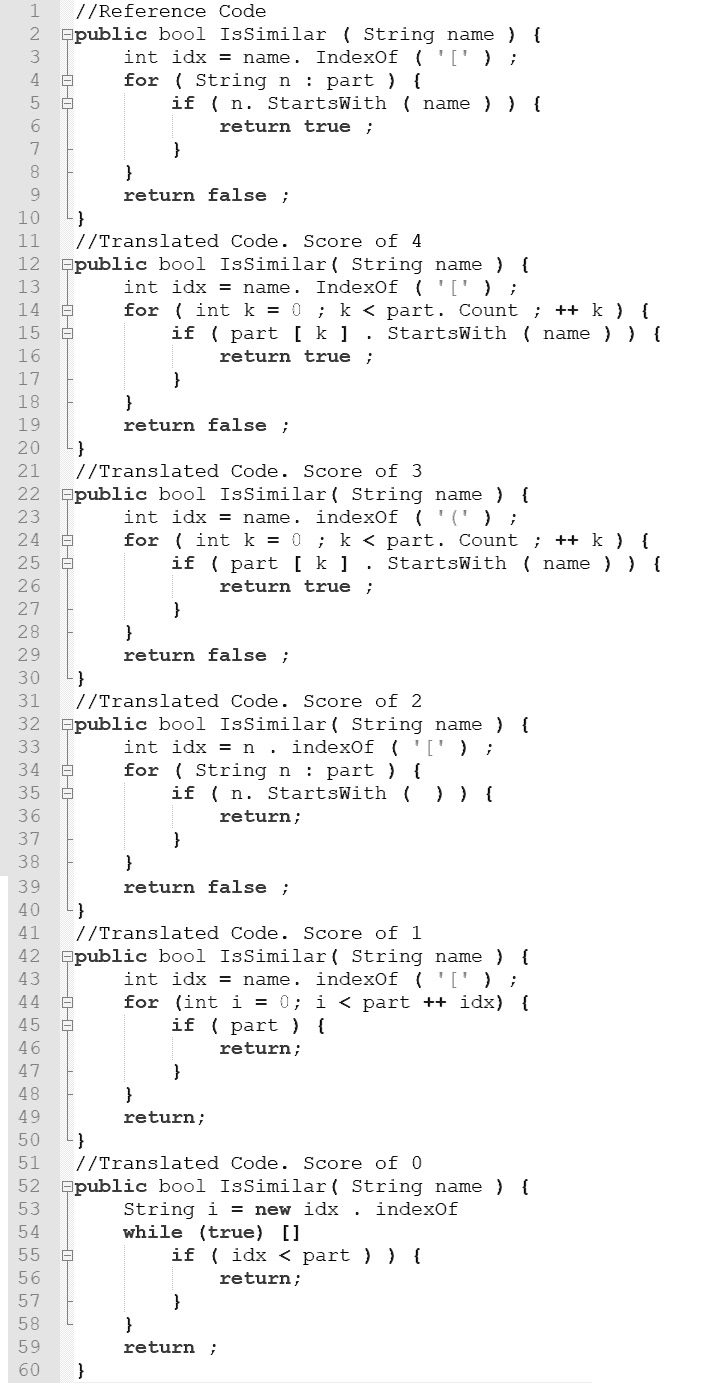
\includegraphics{scoreExamples}

We conducted the same human study for the translated results from all above models with a total of 2,250 manual assignments of such scores. Let us call them \textbf{{\em
    semantic scores}}.


%of both lpSMT and
%mppSMT models. As a result, we have scores for 375 pairs of methods
%for each model. From now on, we regard those scores as \textbf{{\em
%    Semantic score}}.

%\begin{figure}
%\caption{Scoring Examples}
%\centering
%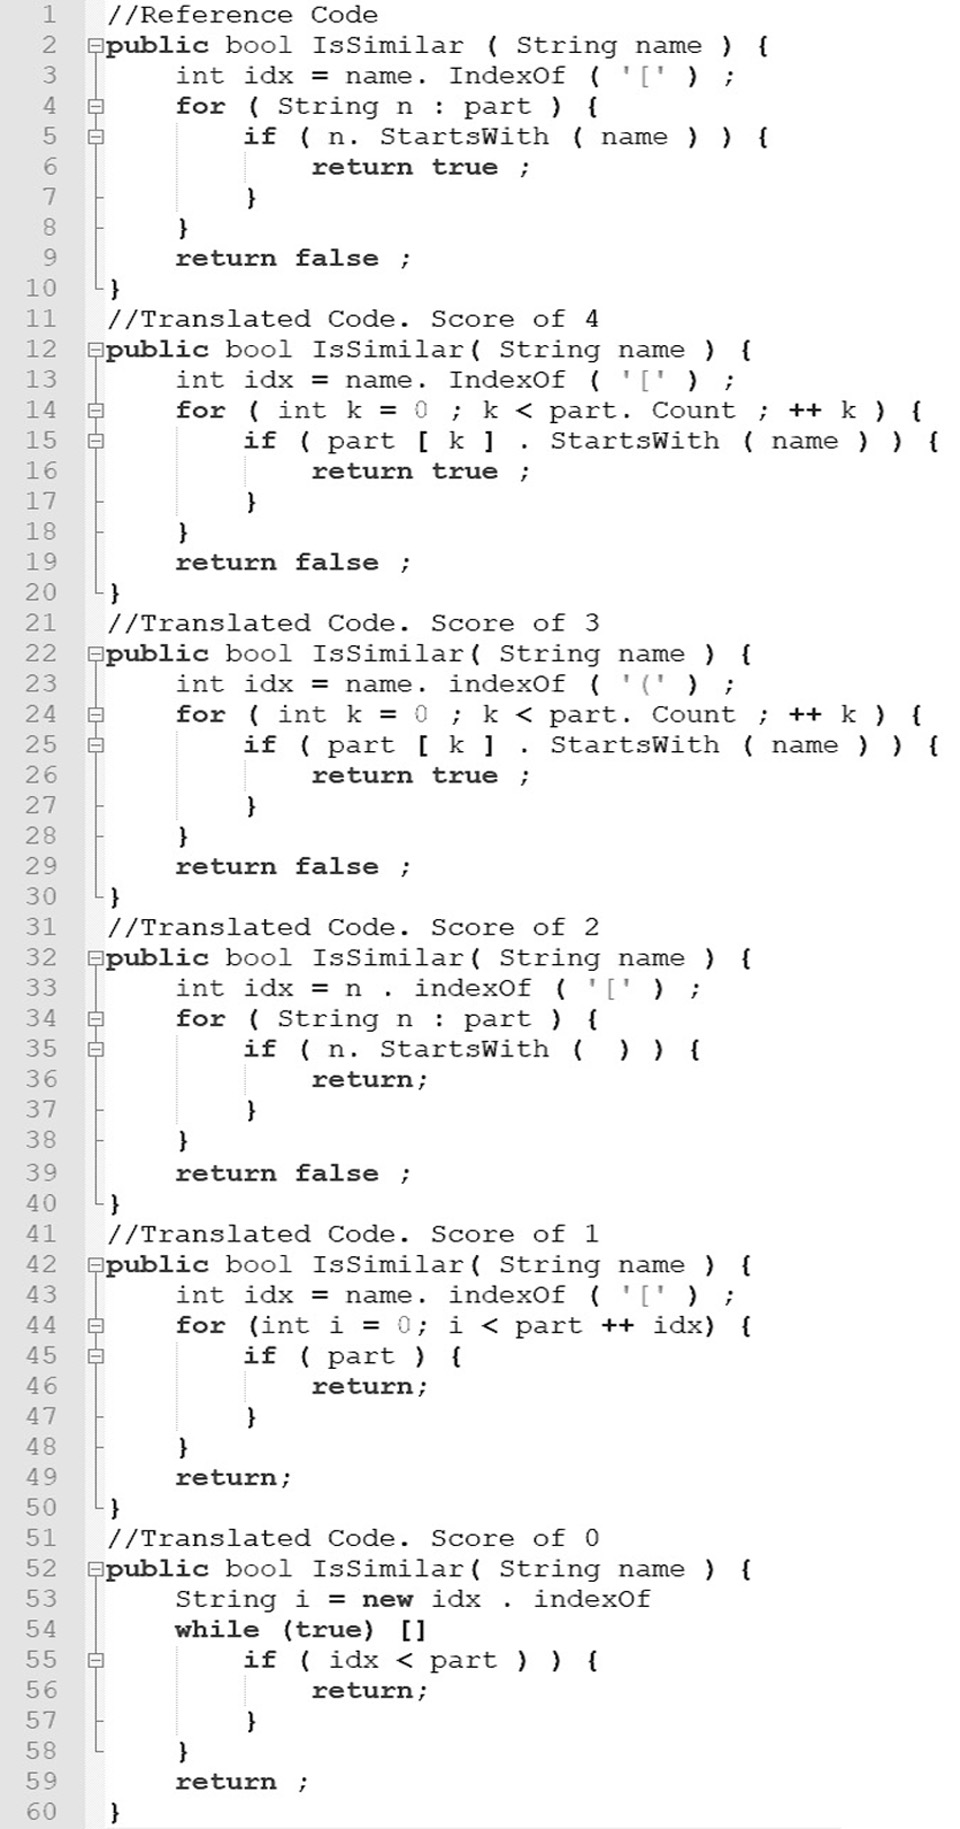
\includegraphics{img/scoreExamples}
%\label{fig:scoreEG}
%\end{figure}


%Our hypothesis states that \emph{\textit{BLEU score does not measure well the similarity in term of semantics between the reference and migrated source code}}. Therefore, given a pair of methods (reference one and machine translated one), we need a metric that can measure the similarity in term of semantics between them. As we know of, there is no automated metrics to do that task. To determine semantic similarity score, we used a human subject to manually evaluate pairs of methods to see how close they are in term of semantic/functionality. Specifically, scoring is done based on the human effort to fix the translated method to achieve the same functionality as of the reference one. The detailed scoring guidelines are presented in Table\ref{table:criteria}. The human subject is a senior developer who is fluent in both Java and C\#. He was given a pair of methods in C\# (machine generated one and reference one), the original method in Java, and the context project from which the methods come from. Then, he was told to evaluate pairs of methods in C\#, and give score as our guideline above and table \ref{table:criteria}. He could also refer back to the original Java method and project for a better understanding of the context. Below are examples for each score from -2 to 2:\\
%To determine semantic similarity score between pair of methods, we manually scored each pair from 0 to 6 based on the human effort to fix a translated method to a referenced one. Specifically, we list the criteria to score in Table  with a score of 0 means the pair of methods are totally different, and a score of 6 means they are totally the same. Scoring also follows the following principles: 1. An effort to fix a syntactical error (misplacing a semi-colon, parenthesis...) has less weight than an effort to fix a semantical error (wrong branch, wrong function call...). 2. A fix that requires adding sources code has more weight than one that requires removing/replacing. 3. A fix for user-defined program elements (identifier, simple name, method name) is more 'pricey' than a fix for keyword (this, if, for...). Example (of scores 1,3,5).

%Since our dataset contains a large number of pairs of methods, it would take a lot of efforts to manually evaluate all of them. Hence, we took a sample from our population of total 34,209 pairs. According to \cite{website}, our sample size is 375 with confidence level of $95\%$ and margin of error $5\%$. After we conducted the human experiment with 375 pairs of methods, we normalized the result on 0-1 range with 0 is respected to -2 and 1 is respected to 2.



\section{Empirical Results}
\label{sec:bleuresult}

In this section, we present the empirical results to validate our hypothesis that 
\textit{BLEU is not effective in evaluating translation quality of source code migration task}
\subsection{Correlation between BLEU and Semantic scores}
To justify the first part of our hypothesis, BLEU score does not reflect well 
the semantic accuracy of results translated by a particular model, 
we show the relation between BLEU scores and human judgments via semantic scores. 
We use Pearson's correlation coefficient~\cite{PearsonCorrelation} to gauge
how strong their relation is. The correlation coefficient has value
between -1 and 1, where 1 indicates the strongest positive relation, -1
indicates the strongest negative relation, and 0 indicates no relation.

Figures~\ref{fig:BleuSemlpSMT} and~\ref{fig:BleuSemMppSMT} show the
scatter plots between two metrics: BLEU and Semantic. Each point
represents the scores of a pair of methods where its $x$-axis value is
for BLEU scores and $y$-axis value is for semantic scores. The
correlation coefficient between BLEU and semantic scores for the model
mppSMT is 0.523 and for the model lpSMT is 0.570. These possitive values 
are closer to 0.5 than to 1.0. This means there is a positive but weak 
relationship between BLEU score and semantic score. The weak correlations %help me to check grammar
between the metrics on the results translated by lpSMT and mppSMT are 
demonstrated in figures~\ref{fig:BleuSemlpSMT} and~\ref{fig:BleuSemMppSMT}.

%\emph{Observation 1:} 
In figure ~\ref{fig:BleuSemlpSMT}, for many specific values of BLEU, it 
is clear that associated semantic scores can be in a wide range. For 
instance, the BLEU score of 0.75, the associated semantic scores are 
from 0.25 to 1 \textbf{Ngoc: can u mark in the figure please}. Thus, from this 
observation, we conclude that the results migrated by certain models 
with high BLEU scores might not archive high semantic scores. 
%There are two reasons for this. 
%

In our sample set, these results can fall in two main cases. 
First, the translated methods might have multiple correct phrases, but in the 
incorrect order, those method can be incorrect, even incompliable.
%useless and justified as so in human judgment.
%
For example, in Figure~\ref{fig:issueexample2}, the translated method
misplaces the position of the bracelet which makes the method has low
Semantic score, but high BLEU score. 
%
%Another reason for this implication is that resulting method does not capture the important
%program elements. 
In other case, the migrated results are incomplete methods missing elements
that are trivial for the translation model, but this violate syntactic rules 
of the target language. For example, the result contains mostly keywords and
punctuation such as \code{if}, \code{public}, \code{()}, but misses
out the important program elements such as function calls or variable
names. In this case, it will have low semantic score while having
a moderate to high BLEU score. These cases indicate the weakness of BLEU metric 
in evaluating the translated results in programing language where syntaxes are well defined.

%\emph{Observation 2:} For a fixed value of Semantic score, there can
%be many associated BLEU values. Specifically, in the model lpSMT, with
%a Semantic Score of 1, the BLEU scores can vary greatly between 0-1,
%which is reflected on the top horizontal line of dots in the
%Figure~\ref{fig:BleuSemlpSMT}. Similarly, in
%Figure~\ref{fig:BleuSemMppSMT}, with the Semantic Score of 1, the BLEU
%scores are in the range of 0.5 to 1.
For the results translated by mppSMT (figure \ref{fig:BleuSemMppSMT}), 
for a particular value of  semantic score, there can be many associated 
BLEU values that spread out over a wide range. Specifically, in the model 
mppSMT, with the absolute semantic score, the BLEU scores can vary greatly 
between 0.5-1. By this empirical results, it can be concluded that for 
some models, the method achieving higher semantic score does not necessarily 
have higher BLEU score. 

%From this observation, it can be implied that translated code can have
%low BLEU score, but high Semantic score. This can be explained by two
%reasons. 
From our sample data, we observe that there are two main reasons leading 
to this phenomenon.
%
First, a translated method can use different code structure from the 
reference one to perform the same functionality. Figure \ref{?} shows an example
that got maximum semantic score, but has low BLEU score (0.4). In this example, 
the translated method uses a \code{for} loop instead of a \code{foreach} 
loop as in the reference code. The second reason causing this phenomenon 
is that the whitespace issue. For example, in figure \ref{?}, the translated method has the 
tokens \code{changeMe()}, but the reference method has \code{changeMe ()}. The former 
is interpreted as one token while the former is interpreted as two tokens. 
This situation reduces the precision on phrases, but the human subject still
evaluated the result with high semantic score. By this experiment, we also empirically 
verify the argument that the forcusing on the lexical precision of BLEU makes
this metric is not able to capture other aspects such as dependencies 
that contribute to the sementics of source code.

%TODO need to verify
In conclusion, BLEU does not reflect well the
semantics of source code, and it is not suitable to use in evaluating
semantic accuracy of a SMT-based code migration system.

\subsection{The Use of BLEU in Comparing Models}
To validate the use of BLEU in comparing different SMT-based code migration systems, we conduct study to see if the change in BLEU scores over models reflect the change in translation quality represented by human judgments of Semantic score. For a same set of 375 original Java methods, the two models GNMT and mppSMT generates two sets of 375 translated methods. Each set has its own BLEU scores and Semantic scores. We ignored pairs of translated results if they have the same BLEU score or Semantic score (136 of the cases). For the remaining results, we found out that in \textbf{34\%} of the cases, the change in BLEU score contradicts the change in Semantic score. It means an improvement in BLEU score leads to a decrease in Semantic score and vice versa. In other words, if one function is translated by two migration models, one-third of the time, the result which has higher BLEU score actually has lower translation quality than the other. Consequently, BLEU is not reliable to use in comparing different SMT-based migration models. 

\begin{figure}
\caption{BLEU metric vs Semantic metric (lpSMT model)}
\centering
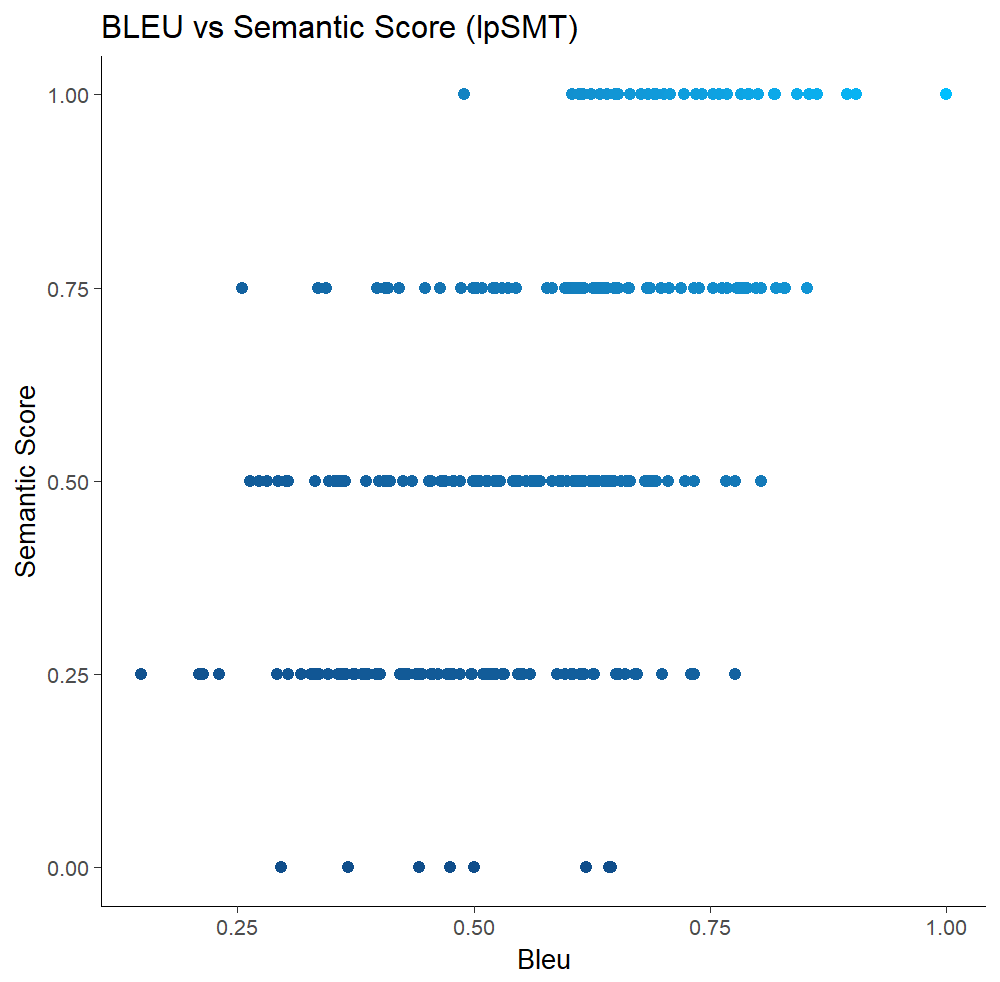
\includegraphics{img/bleuvssemantic_lpSMT.png}
\label{fig:BleuSemlpSMT}
\end{figure}

\begin{figure}
\caption{BLEU metric vs Semantic metric (mppSMT model)}
\centering
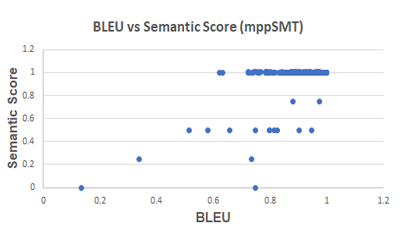
\includegraphics{img/bleuvssemantic_mppSMT.png}
\label{fig:BleuSemMppSMT}
\end{figure}


\section{Alternative metrics}
\label{sec:alternatives}
%Since BLEU did not reflect well the semantic similarity of migrated
%code and reference code, there is a need for an alternative metric
%that can fit better with the task. The nature of the task is to
%compare source code in term of program semantics with respect to a
%programming language.
%
%To compare the two language bases, they must be represented in some
%ways. 

As Section~\ref{sec:bleuresult} shows that BLEU is ineffective in
evaluating translated code, in this section, we will present our
evaluation on the effectiveness of various other metrics. The
effectiveness of a metric is expressed in its abilities to measure the
similarity between the reference code and the migrated code in term of
program semantics according to a programming~language.

%SON: How about the abilities to evaluate the translation quality improvement of models
%While a language is normally composed by three important parts:
%vocabulary, grammar, and meaning; programming language can be composed
%by the three corresponding parts: lexeme, syntax, and semantics. 

In general, a programming language can be characterized by three
important parts: lexeme, syntax, and semantics that are corresponding
with three important parts in a natural language: vocabulary, grammar,
and meaning.
%Therefore, we consider three representations: tokens, abstract syntax trees
%(ASTs), and program dependence graphs (PDGs) that reflect each of the
%three above parts respectively. 
These parts of a programming language could be represented respectively in three 
abstractions: tokens (text), abstract syntax tree (AST), and program 
dependence graph (PDG).
%
There are a number of clone detection approaches~\cite{clone-tse07},
which are token-based~\cite{ccfinder},
tree-based~\cite{baxter98,deckard}, and PDG-based~\cite{deckard2} to
measure the similarity of source code in these three representations.
These techniques have shown that the duplication of source code in
term of functionality can be detected more precisely when the higher
level representations are applied from text, AST, to
PDG~\cite{clone-tse07,deckard2}.
%The higher level of representation is
%used, the higher type of cloned code the technique can detect.
%The key rationale is that The cause of this precision might be
%the more semantics information that is stored by the higher
%abstraction level of source code. 
Based on that, we have the following hypothesis: \textit{the metric
  that measures results in the higher abstraction level reflects
  better the similarity of the translated code and the reference one
  in term of program semantics}.

%Comparing source code by using those 
%representations would give us three metrics to measure semantics similarity. 
%Each representation would reflect semantics of source code in certain ways.
%For example, a pair of methods that have identical lexemes would have 
%identical program semantics, but if they are different in term of lexeme, 
%it is uncertain to determine their semantic similarity. Therefore, to fully 
%capture how well these representations reflect semantics accuracy, it is 
%necessary to conduct empirical study that measures the correlation between 
%each metric with semantic score graded by human expert.
%choose one representation for each of the above part to
%compare, in order to heuristically estimate the semantic
%similarity. 
%Specifically, token, AST and PDG are representations of lexemes,
%syntax, and semantics respectively. 
%
%Let us explain the metrics to compare the three above representations.
%
%The metrics to compare those representations are SED, TREED and GVED
%which are defined below. Those metrics are then evaluated to show how
%well they reflect Semantic score.
To validate the hypothesis, we conduct our experiments to evaluate the
effectiveness of three metrics: \textbf{string similarity},
\textbf{tree similarity}, and \textbf{graph similarity} that measure
the results in the text, tree and graph representations for code
respectively, in reflecting the semantic accuracy of translated
results.

\subsection{Code similarity metrics}

In this work, we define the similarity scores on token-based,
tree-based and graph-based representations between the translated
result and the reference code as the inverse of string edit
distance~\cite{levenshtein}, tree edit distance~\cite{oopsla10}, and graph edit
distance~\cite{sanfeliu}, respectively.

\textbf{String similarity (STS)} is the metric to compare the
similarity of source code that is represented as sequence of
tokens. The similarity between the translated result $T$ and its
reference code $R$ is computed as:
$$STS(R, T) = 1 - \frac{SED(S_R, S_T)}{max\left(length(S_R), length(S_T)\right)}$$
where $SED(S_R, S_T)$ is the string edit distance between the
reference sequence $S_R$ and the translated sequence $S_T$, that
measures efforts that a user must edit in term of the tokens that need
to be deleted/added to transform the resulting code into the correct one;
$length(t)$ refers to the length of the sequence~$t$.

%For example, $EditDistance\left(s_R, s_T\right)$ between translated code and
%reference code in Figure~\ref{fig:issueexample2} is 4 (two deletions,
%two additions). Then, it is normalized as 0.952. Note that the closer
%the score to 1, the more similar the pair in term of lexical~tokens.

%Abstract syntax tree (AST) is the most widely-used representation in
%representing the syntactic structures in source code. Therefore,
%computing the difference of two ASTs is considered as evaluating
%syntactic difference.  In our study, we apply this idea in measuring
%the difference between the syntactic structures of reference code and
%translated code. Given a pair of methods in C\# which are need to be
%syntactically compared, we used Roslyn~\cite{roslyn} to parse them into
%ASTs. Then, we compute the tree edit distance between two trees using
%the algorithm Treed~\cite{oopsla10}. Specifically, the tree edit
%distance is calculated by number of operations ({\em add}, {\em
%delete}, {\em replace}, and {\em move}) to make them identical.

\textbf{Tree similarity (TRS)} is the metric used to measure
the similarity between two ASTs representing for the translated code ($T$)
and the reference one ($R$):
$$TRS(R, T) = 1 -\frac{TED(AST_R, AST_T)}{max\left(size(AST_R),
  size(AST_T)\right)}$$ where $TED(AST_R, AST_T)$ is the edit
distance between the ASTs of the reference code $AST_R$ and the
translated code $AST_T$, which is calculated by the minimum number of
editing operations on AST nodes ({\em add}, {\em delete}, {\em
  replace}, and {\em move}) to sequentially make $AST_R$ and $AST_T$
identical \cite{oopsla10}; and $size(t)$ returns the number of
nodes in the AST $t$.
%
%For any two trees, there will always exist at least one editing (such
%as the one that deletes all the nodes of the first tree and inserts all
%the nodes of the second). Therefore, there will always exist at least
%one TREED value and the higher value it is, the more similar those
%trees are.
%
%\begin{figure}[h]
%	\caption{Tree Editing Example: In the label of each node, its type is in capital font and its val (if exists) is in normal font}
%	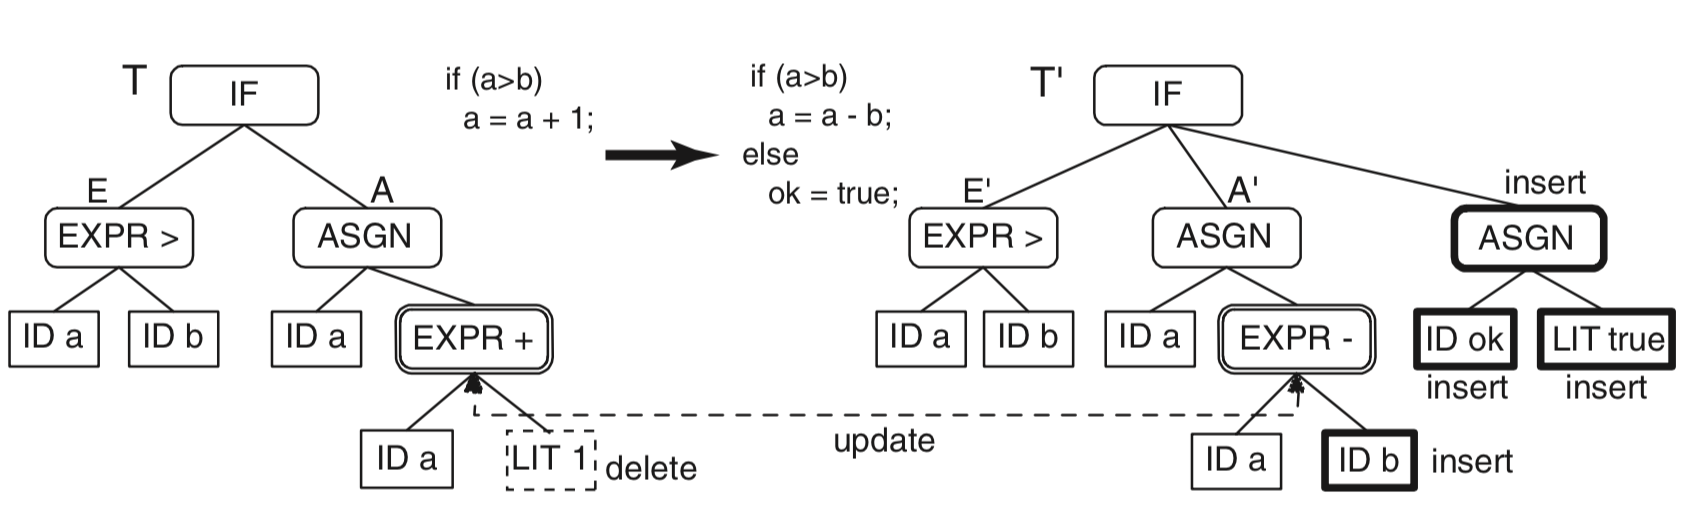
\includegraphics[scale=0.3]{img/treed.png}
%	\centering
%	\label{fig:treed}
%\end{figure}
%
%In the example in Figure \ref{fig:treed}, an \textit{if} statement was
%edited by modifying the \textit{if} branch and adding an \textit{else}
%branch. The two ASTs represent the two versions of a method. An edit
%consists of one \textit{Delete} (dotted line box), one \textit{Update}
%(double-line box), and four \textit{Insert} operations (bold
%boxes). Other nodes (single- line boxes) are either unchanged or
%moved. Based on the formula of TREED, the result in this case is:
%$TREED = 1 - \frac{1 + 1 + 4}{16}=0.625$.

%\subsubsection{\textbf{Graph Vector Edit Distance (GVED)}}
%
%Graph-based approaches in representing program semantics have become
%popular. Among those approaches, PDGs are one of the most popular.  To
%capture the graph structures in PDGs, we choose Exas~\cite{fase09}.
%Exas is an efficient structural characteristic feature extraction
%approach that approximates and captures the structure within the
%fragments of artifacts~\cite{fase09}.  In our study, we use Exas as a
%mean of computing the difference between two PDGs. Given a pair of
%method in C\# which are need to be compared, their respective
%(PDGs) are built.
%% with some additional nodes from GROUM~\cite{fse09}.
%Exas vectors will be computed on those graphs. In Exas, the
%characteristic features are extracted from the patterns of elements of
%the graphs. The code fragments are characterized by their counting
%vectors of those features. The difference between two vectors reflects
%the difference of two graphs.

%TODO cite Sanfeliu, Alberto; Fu, King-Sun (1983). "A distance measure between attributed relational graphs for pattern recognition"
In this work, we define \textbf{graph similarity (GRS)} between the
translated result $T$ and the reference code $R$ represented as PDGs
by using graph edit distance~\cite{sanfeliu}. That is:
$$GRS(R, T) = 1-\frac{GED(PDG_R, PDG_T)}{max\left(size(PDG_R),
  size(PDG_T)\right)}$$ where $GED(PDG_R, PDG_T)$ is the edit distance
between the PDG of the reference code $PDG_R$ and the PDG of the
translated code $PDG_T$; $size(g)$ is the sum of the number of
vertexes and edges of the graph $g$. Specifically, $GED(PDG_R, PDG_T)$
is computed as the minimum number of graph edit operations to
transform one graph to another. The feasible graph edit operations on
vertexes and edges includes {\em insert}, {\em delete}, and {\em
  substitute}.  However, computing the graph edit distance between two
graphs is NP-hard.  In this work, we use Exas~\cite{fase09}, a highly
precise approximate technique to compute $GED$.


%Therefore, distance of these counting vectors is considered the way to measure the sematic between code fragments.

%Figure~\ref{fig:PDGs} shows the PDGs of the code fragments 1 and
%2. These graphs are analysed by Exas, which focuses on two kinds of
%patterns of structural information of the graph, called $\left(p,q\right)$-node
%and $n$-path as can be seen in Table~\ref{tab:feature1} and
%Table~\ref{tab:feature2}.
%
%An efficient way to express the property ``having the same or similar
%features'' is to use vectors. The characteristic vector of a fragment
%is the occurrence-count vector of its features. That is, each position
%in the vector is indexed for a feature and the value at that position
%is the number of occurrences of that feature in the
%fragment. Table~\ref{tab:featureIndex} shows the indexes of the
%features, which are global across all vectors. Based on the occurrence
%counts, the vectors for code fragment 1 and~2 are
%$V_1$(1,1,1,1,1,0,1,0...) and $V_2$(1,1,0,1,1,1,1,1...),
%respectively. Two fragments having the same feature sets and
%occurrence counts will have the same vectors. The
%vector similarity can be measured by a chosen vector distance such as
%1-norm distance.
%
%We introduce the formula for normalizing the result of vector edit
%distance which is used in our experiments. The normalized
%value is described as
%\[GVED \left( V_1, V_2 \right) = 1 - \sum_{i=1}^{n} \frac{ \mid XV1_i - XV2_i \mid}{XV1_i + XV2_i}\]
%where $n$ denotes the number of vector scalar, $V_1$ denotes the
%counting vector of the first graph, $V_2$ denotes the counting vector
%of the second graph; $XV1_i$ denotes the value of the ($i-th$) scalar
%of $V_1$; and $XV2_i$ denotes the value of the ($i-th$) scalar of
%$V_2$.
%
%In this example in Figure~\ref{code1code2}, the value of GVED is
%$GVED\left(V_1, V_2\right) = 1 - \frac{8 }{20} = 0.6 $.
%
%\begin{figure}
%\begin{lstlisting}[language=JAVA]
%	Code 1:
%	void foo(int i) {
%		int j;
%		if (i < 2) {
%			j = 1;
%		} else {
%			j = 2;
%		}
%	}
%
%	Code 2:
%	void foo(int i) {
%		int j;
%		if (i < 2)
%			j = i;	
%		j = 2;
%	}
%\end{lstlisting}
%\caption{Example of two code fragments}
%\label{code1code2}
%\end{figure}
%
%\begin{figure}[t]
%	\caption{An example: two PDGs represent code fragments 1 and 2}
%	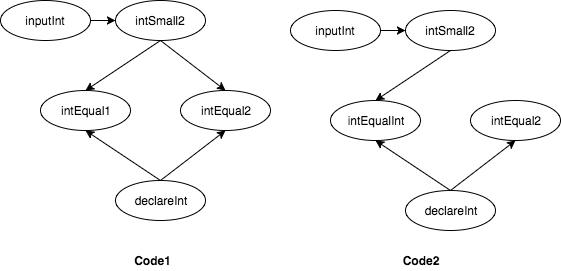
\includegraphics[scale=0.4]{img/Diagram_PDG.png}
%	\centering
%	\label{fig:PDGs}
%\end{figure}
%
%% Table generated by Excel2LaTeX from sheet 'Sheet1'
%\begin{table}[t]
%  \centering
%  \caption{Feature Table of Code Fragment 1 in Exas}
%  \scalebox{0.65}{
%    \begin{tabular}{|l|l|l|l|l|r|}
%    \toprule
%    \textbf{Pattern} & \multicolumn{5}{c|}{\textbf{Feature of Code1}} \\
%    \midrule
%    \textit{\textbf{1-path}} & inputInt & intSmall2 & intEqual1 & intEqual2 & \multicolumn{1}{l|}{declareInt} \\
%    \midrule
%    \textit{\textbf{2-path}} & \multicolumn{1}{p{6.415em}|}{inputInt-intSmall2} & \multicolumn{1}{p{5.915em}|}{intSmall2-intEqual1} & \multicolumn{1}{p{6em}|}{intSmall2-intEqual2} & \multicolumn{1}{p{5.75em}|}{declareInt-intEqual1} & \multicolumn{1}{p{5em}|}{declareInt-intEqual2} \\
%    \midrule
%    \textit{\textbf{3-path}} & \multicolumn{1}{p{6.415em}|}{intputInt-intSmall2-intEqual1} & \multicolumn{1}{p{5.915em}|}{intputInt-intSmall2-intEqual2} &       &       &  \\
%    \midrule
%    \textit{\textbf{(p,q)-node}} & inputInt-0-1 & intSmall2-1-2 & intEqual1-2-0 & intEqual2-1-2 &  \\
%    \bottomrule
%    \end{tabular}%
%	}
%  \label{tab:feature1}%
%\end{table}%
%
%% Table generated by Excel2LaTeX from sheet 'Sheet1'
%\begin{table}[t]
%  \centering
%	\caption{Feature Table of Code Fragment 2 in Exas}
%	\scalebox{0.65}{
%	    \begin{tabular}{|l|l|l|l|l|r|}
%    \toprule
%    \textbf{Pattern} & \multicolumn{5}{c|}{\textbf{Feature of Code2}} \\
%    \midrule
%    \textit{\textbf{1-path}} & inputInt & intSmall2 & intEqualInt & intEqual2 & \multicolumn{1}{l|}{declareInt} \\
%    \midrule
%    \textit{\textbf{2-path}} & \multicolumn{1}{p{6.415em}|}{inputInt-intSmall2} & \multicolumn{1}{p{5.915em}|}{intSmall2-intEqualInt} & \multicolumn{1}{p{6em}|}{declareInt-intEqual1} & \multicolumn{1}{p{5.75em}|}{declareInt-intEqual2} &  \\
%    \midrule
%    \textit{\textbf{3-path}} & \multicolumn{1}{p{6.415em}|}{intputInt-intSmall2-intEqualInt} &       &       &       &  \\
%    \midrule
%    \textit{\textbf{(p,q)-node}} & inputInt-0-1 & intSmall2-1-1 & intEqualInt-2-0 & intEqual2-1-0 &  \\
%    \bottomrule
%    \end{tabular}%
%	}
%  \label{tab:feature2}%
%\end{table}%
%
%% Table generated by Excel2LaTeX from sheet 'Sheet1'
%\begin{table}[htbp]
%	\centering
%	\caption{Feature Indexing}
%	\scalebox{0.75}{
%	\begin{tabular}{|cccc|}
%		\toprule
%		\multicolumn{1}{|l|}{\textbf{Feature}} & \multicolumn{1}{l|}{\textbf{Index}} & \multicolumn{1}{l|}{\textbf{Counted in Code1}} & \multicolumn{1}{l|}{\textbf{Counted in Code2}} \\
%		\midrule
%		\multicolumn{1}{|l|}{inputInt} & \multicolumn{1}{r|}{1} & \multicolumn{1}{r|}{1} & \multicolumn{1}{r|}{1} \\
%		\midrule
%		\multicolumn{1}{|l|}{intSmall2} & \multicolumn{1}{r|}{2} & \multicolumn{1}{r|}{1} & \multicolumn{1}{r|}{1} \\
%		\midrule
%		\multicolumn{1}{|l|}{intEqual1} & \multicolumn{1}{r|}{3} & \multicolumn{1}{r|}{1} & \multicolumn{1}{r|}{0} \\
%		\midrule
%		\multicolumn{1}{|l|}{intEqual2} & \multicolumn{1}{r|}{4} & \multicolumn{1}{r|}{1} & \multicolumn{1}{r|}{1} \\
%		\midrule
%		\multicolumn{1}{|l|}{declareInt} & \multicolumn{1}{r|}{5} & \multicolumn{1}{r|}{1} & \multicolumn{1}{r|}{1} \\
%		\midrule
%		\multicolumn{1}{|l|}{intEqualInt} & \multicolumn{1}{r|}{6} & \multicolumn{1}{r|}{0} & \multicolumn{1}{r|}{1} \\
%		\midrule
%		\multicolumn{1}{|p{5.75em}|}{inputInt-intSmall2} & \multicolumn{1}{r|}{7} & \multicolumn{1}{r|}{1} & \multicolumn{1}{r|}{1} \\
%		\midrule
%		\multicolumn{1}{|l|}{intEqual2-1-0} & \multicolumn{1}{r|}{8} & \multicolumn{1}{r|}{0} & \multicolumn{1}{r|}{1} \\
%		\midrule
%		\multicolumn{4}{|c|}{To be continued} \\
%		\bottomrule
%	\end{tabular}%
%	}
%	\label{tab:featureIndex}%
%\end{table}%





 
\subsection{Experimental results on alternative metrics}

%To further study the relations between each of the three above metrics
%and the semantic scores, we conducted several experiments in the same
%manner as the previous study described in
%Section~\ref{sec:bleuresult}. We then present our proposed metric
%in Section~7 based on the results of the following experiments.

To evaluate the abilities of STS, TRS and GRS in reflecting the
semantic accuracy of translated code, we conducted three experiments
for these three metrics in the same manner as the study described in
Section~\ref{sec:bleuresult}.

The correlation coefficient results between each of the three metrics
with semantic score are described in
Table~\ref{table:correlation}. These results follow a similar trend:
for each model, the correlation coefficients increase 
according the abstraction levels of source code from text, syntax, to semantic
representations in three metrics. For example, for mppSMT, the correlation
coefficient between STS and semantic score is 0.549, whereas that
for TRS is much greater at 0.820. The highest value is the
correlation coefficient between GRS and semantic score at 0.910. A
reason for this phenomenon is that for a pair of source code, if they
are textually identical, they have the same AST representation, and
the exact-match in AST leads to the equivalence between the
corresponding PDGs. Meanwhile, the equivalence in a higher
abstraction level does not necessarily lead to the equivalence in a
lower abstraction. For example, Fig.~\ref{fig:mppSMT_example} shows
two methods with equivalent PDGs, but with textually~different. 

%Despite of the increase of the correlation coefficients, GRS and TRS
%are used to measure subsets of methods in our sample set 
%(table \ref{table:metrics}), and the sizes of GRS are greater than 
%TRS's ones, whereas STS is able to apply for all cases. For example, 
%the applicable sets of methods translated by lpSMT are quite limited, 
%75 and 123 (out of 375 methods) for GRS and TRS respectively. The reason
%for this phenomenon is that to construct the higher level representations,
%the translated results need to satisfy certain syntactic and semantic related
%constraints such as resolvable data and control dependencies.
%\begin{table}
%\centering
%\caption{Numbers of applicable methods of metrics}
%\begin{tabular}{|c|c|c|}
%\hline
%  & GRS & TRS\\
%\hline
%GNMT  & 128 & 155  \\
%\hline
%mppSMT  & 239 & 292 \\
%\hline
%lpSMT & 75 & 123 \\
%\hline
%\end{tabular}
%\label{table:metrics}
%\end{table}

Based on these empirical results, we conclude that the metric that
measures the results in the higher abstraction level, the better
metric for reflecting the semantics accuracy. However, the higher
representation like PDG cannot always be constructed because of
missing syntactic or semantic related information in the translated
results that is required to construct ASTs and PDGs. For example, the
sets of methods that are translated by lpSMT, and applicable for GRS
and TRS are quite limited, 75 and 123 (out of 375 methods),
respectively (the respective numbers for mppSMT are 239 and 292, and
those for GNMT are 128 and 155). Therefore, in
Section~\ref{sec:proposal}, we propose a metric to evaluate the
quality of translated code, that uses the measurement of the
similarity of translated code and expected results in multiple
representations.

%It is not worth to use SED instead of BLEU since it still has the same
%problems as BLEU while its advantage is insignificant.
%We then present our proposed metric in section~7 based on the results of the following experiments.

%To verify the 3 metrics SED, TREED, and GVED , we conducted an exploratory study that reveals their correlation with the ground truth Semantic score. Table \ref{table:correlation} summarizes our results for the two models mppSMT and lpSMT. We will explain each metric \rq s correlation in details as follows:

\begin{table}
\centering
\caption{Correlation between each metric with  semantic score on three models}
\begin{tabular}{|c|c|c|c|c|}
\hline
 & STS & TRS & GRS\\
\hline
mppSMT  & 0.549 & 0.820 & 0.910 \\
\hline
lpSMT  & 0.533 & 0.786 & 0.823 \\
\hline
GNMT & 0.692 & 0.734 & 0.927 \\
\hline
\end{tabular}
\label{table:correlation}
\end{table}


%\subsubsection{\textbf{SED vs Semantic}}
%
%SED is similar to BLEU in the way that both of them compare source
%code in term of lexical representation. Indeed, the two metrics have
%similar correlations with Semantic score
%(Table~\ref{table:correlation}). The correlation coefficient between SED and Semantic score is 0.549,
% 0.533, and 0.692 for three models mppSMT, lpSMT, and GNMT respectively.
%%equivalent 0.523 and 0.549 (mppSMT), and 0.67 and 0.675 (lpSMT). SED
%SED suffers the same drawbacks as BLEU: it does not take into
%consideration the structures of source code, and it compares source
%code only in term of lexical tokens.
%It is not worth to use SED instead of BLEU since it still has the same
%problems as BLEU while its advantage is insignificant.

%\begin{figure}
%\caption{SED vs Semantic (lpSMT)}
%\centering
%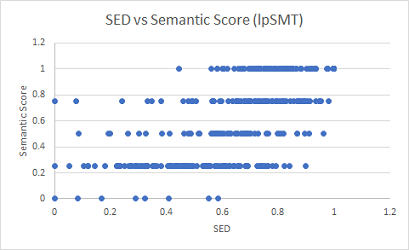
\includegraphics{img/sedvssem_lpSMT.png}
%\label{fig:SedSemlpSMT}
%\end{figure}
%
%\begin{figure}
%\caption{SED vs Semantic (mppSMT)}
%\centering
%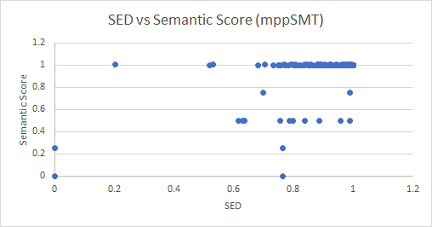
\includegraphics{img/sedvssem_mppSMT.png}
%\label{fig:SedSemMppSMT}
%\end{figure}

%\subsubsection{\textbf{TREED vs Semantic}}
%TREED compares source code at higher level of representation (Syntax Tree). Syntax of source code is the pre-requisite before mentioning about its semantics or functionality. Comparing methods in term of syntax is likely to reflect semantic accuracy better than comparing at lexical level. This argument is proved by our empirical results:

%Technically, a translated method cannot be said to perform any functionality if it cannot be compiled. However, in the Code Migration problem, a translated method which has wrong syntax can still be useful for developers.

%Figure \ref{fig:TREEDmppSMT} shows the scatter plots between 2
%metrics: TREED and Semantic score for the model mppSMT. In general, the result has similar
%trend as in the relation of BLEU and Semantic score: the data points
%are too scattered to show a strong correlation and there are
%several outliers. For a fixed value of Semantic score, TREED score can
%still vary in a large range. However, compared to BLEU, the variation
%is much smaller. For example, a pair of method that has Semantic score
%of 0.5 can possibly have TREED scores in range of 0.7 to 1 while such
%range is 0.5 to 1 for BLEU. TREED shows noticeable improvement over
%BLEU or SED on the correlation with Semantic score on the mppSMT model
%(0.549 to 0.820), on lpSMT model (0.533 to 0.786), and on the GNMT model (0.692 to 0.734).

%\emph{Observation 1:} For a fixed value of Semantic score, there can be many associated TREED values. Specifically, in the model lpSMT, with a Semantic Score of 1, the TREED scores can be varied greatly between 0-1, which was reflected on the top horizontal line of dots in figure \ref{fig:TREEDlpSMT}. Similarly, in the figure \ref{fig:TREEDmppSMT}, with a Semantic Score of 1, the TREED scores are in the range of 0.7 to 1.
%
%\emph{Observation 2:} For a fixed value of TREED, there can be many associated Semantic scores. For example, the figure \ref{fig:TREEDlpSMT} shows that for a high TREED score, for example 0.8, can have Semantic Score from 0.25 to 1. This can be observed by the vertical line of dots in the figure.



% Comparing figure \ref{fig:BleuSemMppSMT} and figure \ref{fig:TREEDmppSMT}, it can be realized that on the model mppSMT, those horizontal lines of dots in figure \ref{fig:BleuSemMppSMT} became shorter in figure \ref{fig:TREEDmppSMT}. It means the variation of TREED score for certain Semantic score is lower. Data points in the figure can also be approximately fitted with a regression line even though there still are some outliers.

%From observation 1, it can be implied that a translated method can have low TREED score, but high Semantic score. On the other hand, from observation 2, a translated method can have high TREED score, but low Semantic score. The two implications above shows that an improvement in TREED is not sufficient nor necessary to improve translation migration quality. However, from observation 3, there is hint of positive improvement that using TREED would reflect Semantic score better than BLEU.

%Issues of TREED that were showed by the figure \ref{fig:TREEDmppSMT} can be explained by two reasons. First, a translated method can be syntactically correct, however still does not have the same functionality as the reference
%code (high TREED score, low Semantic score). Secondly, there
%exists the scenarios of low TREED score with high Semantic score. For
%example, a translated method can have an incorrect place for a
%semicolon, which makes it not compiled. Beside that mistake, if it can
%reflect the functionality of the reference code, it still has a high
%Semantic score. However, due to the increase of coefficient, there is
%an indication that TREED would reflect syntactic correctness better
%than BLEU.

%In certain circumstance, TREED could be used to evaluate SMT-based
%Migration system that focuses on translating correct syntax code.

%\begin{figure}
%\caption{TREED vs Semantic (lpSMT)}
%\centering
%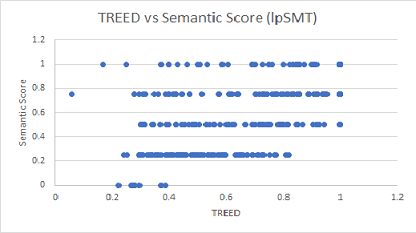
\includegraphics{img/treed_lpSMT.png}
%\label{fig:TREEDlpSMT}
%\end{figure}
%
%\begin{figure}
%\caption{TREED vs Semantic (mppSMT)}
%\centering
%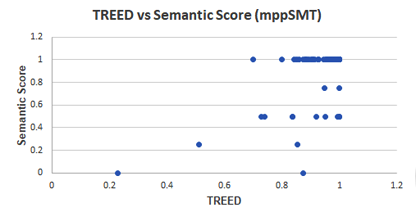
\includegraphics{img/treed_mppSMT.png}
%\label{fig:TREEDmppSMT}
%\end{figure}
%
%\subsubsection{\textbf{GVED vs Semantic}}

%There are studies that compare PDGs to measure the semantic
%similarity. PDGs capture all data and control dependence of program
%elements, and those dependencies are the keys to reflect functionality
%of source code. Therefore, GVED is expected to have the best
%correlation with Semantic score. Our results cement this argument.

%Figure \ref{fig:GVEDmppSMT} shows the scatter plots between 2 metrics:
%GVED and Semantic score when GVED is applicable. There are 240 of such
%points for the model mppSMT in the total of 375 pairs of methods, and
%75 points for lpSMT, respectively. The correlation coefficients between
%GVED and Semantic score are 0.910, 0.823, and 0.927 for the 3 models mppSMT, lpSMT, and GNMT respectively. These values show the better correlations with
%Semantic score than any of the BLEU, SED, and TREED metrics.
%
%significant improvements on both models comparing to any of the other
%3 metrics.
%
%All other three metrics have correlation coefficients with Semantic
%Score less than 0.7 while GVED achieves remarkable correlation
%coefficients of nearly 1.0 .
%
%GVED's promising result makes it an obvious choice to evaluate
%SMT-based Code Migration systems.
%

%A caveat to this is that not all migrated code is sufficiently correct
%to build the corresponding PDGs.
%
%the translated methods have too many errors that cannot be built into
%PDG, or even be compiled.
%That explains the situation in which the number of data points
%available for model lpSMT is too small to draw conclusion about the
%correlation with high confidence. Therefore, even though GVED is a
%metric with highest correlation with Semantic scores, it is not always
%applicable. To cope with its limitation while still utilizing its
%strength in correlation with semantic scores, we explore the
%combination of GVED and other metrics in our novel metric, {\model}.


%\begin{figure}
%\caption{GVED vs Semantic (lpSMT)}
%\centering
%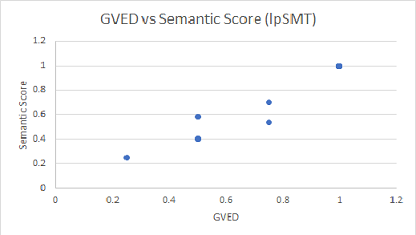
\includegraphics{img/gved_lpSMT.png}
%\label{fig:GVEDlpSMT}
%\end{figure}
%
%\begin{figure}
%\caption{GVED vs Semantic (mppSMT)}
%\centering
%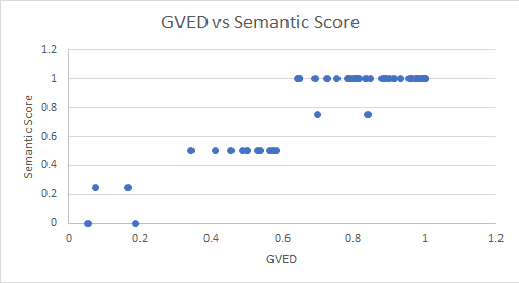
\includegraphics{img/gved_mppSMT.png}
%\label{fig:GVEDmppSMT}
%\end{figure}


\section{Proposal}
\subsection{\model}
%For a SMT-based migration system, BLEU has always been like this... doing that....

%From the results in section 5, BLEU did not reflect the semantic accuracy of source code. --> We need a better metrics to replace BLEU

%Needed metric should be 
%Reflect semantical meaning of sources code.
%Automated
%Low computation's cost
%Independent of programming language
%Independent of MT model's type

Considering all those requirements above, we introduce {\model}, a novel automated metric that can reflect semantic accuracy of translated code. {\model} is also independent of programming languages and machine translation models used in migration system. {\model} measures the semantic accuracy of the resulting code by comparing the program dependence graph (PDG) between them. PDG captures both the data and control dependencies among program entities. Because of its properties, we expect PDG can represent well the semantic level of source code. To reduce the high computational cost, we vectorize the PDG and calculate the vector difference to estimate the graph difference. This way, we would make sure that our model is practical and applicable in large scaled systems. 

When applying MT on source code, there always exists the problem that the translated code is not compilable. Thus, it is impossible to build PDG on those code. To cope with the problem, our model is designed as best-effort, layered metric  : If the translated code can be built into PDG, we calculate {\model} in term of graph difference. If the translated code cannot be built into PDG but is compilable, we calculate {\model} in term of syntax tree edit distance. If the translated code is not compilable, we calculate {\model} in term of string edit distance. 

if (GVED(s,t) != -1) RUBY(s,t) = GVED(s,t)\\
else if (TREED(s,t) != -1) RUBY(s,t) = TREED(s,t)\\
else RUBY(s,t) = SED(s,t)
\section{Related Work}

There exist
many studies aiming to measure the functionality similarity of source
code, which utilize the similarities of structures and
dependencies~\cite{clone-tse07,roy09,baker97,ccfinder,cpminer,deckard,deckard2,horwitz01}.
%baxter98,ducasse99
However, they are not reliable as their results sometimes contradict
with human judgments on semantic accuracy~\cite{deckard2}.

However, there exists criticism on BLEU
as Callison-Burch {\em et al.}~\cite{Callison} argued that an
improvement in BLEU metric is not sufficient nor necessary to show an
improvement in translation quality. Despite such criticism,

\section{Conclusion}

% Note that the IEEE does not put floats in the very first column
% - or typically anywhere on the first page for that matter. Also,
% in-text middle ("here") positioning is typically not used, but it
% is allowed and encouraged for Computer Society conferences (but
% not Computer Society journals). Most IEEE journals/conferences use
% top floats exclusively. 
% Note that, LaTeX2e, unlike IEEE journals/conferences, places
% footnotes above bottom floats. This can be corrected via the
% \fnbelowfloat command of the stfloats package.




%\section{Conclusion}
%The conclusion goes here.




% conference papers do not normally have an appendix


% use section* for acknowledgment
%\section*{Acknowledgment}


%The authors would like to thank...





% trigger a \newpage just before the given reference
% number - used to balance the columns on the last page
% adjust value as needed - may need to be readjusted if
% the document is modified later
%\IEEEtriggeratref{8}
% The "triggered" command can be changed if desired:
%\IEEEtriggercmd{\enlargethispage{-5in}}

% references section

% can use a bibliography generated by BibTeX as a .bbl file
% BibTeX documentation can be easily obtained at:
% http://mirror.ctan.org/biblio/bibtex/contrib/doc/
% The IEEEtran BibTeX style support page is at:
% http://www.michaelshell.org/tex/ieeetran/bibtex/
%\bibliographystyle{IEEEtran}
% argument is your BibTeX string definitions and bibliography database(s)
%\bibliography{IEEEabrv,../bib/paper}
%
% <OR> manually copy in the resultant .bbl file
% set second argument of \begin to the number of references
% (used to reserve space for the reference number labels box)
%\begin{thebibliography}{1}

%\bibitem{IEEEhowto:kopka}
%H.~Kopka and P.~W. Daly, \emph{A Guide to \LaTeX}, 3rd~ed.\hskip 1em plus
%  0.5em minus 0.4em\relax Harlow, England: Addison-Wesley, 1999.

%\end{thebibliography}

\newpage

\balance
%\bibliographystyle{abbrv}
%\citestyle{acmauthoryear}

\bibliographystyle{IEEEtran}

%\setcitestyle{numbers,sort&compress}
\bibliography{ase18}


% that's all folks
\end{document}


